\documentclass[11pt]{article}

% \usepackage[preprint]{acl}
\usepackage[preprint]{acl}
\usepackage{times}
\usepackage{latexsym}
\usepackage[T1]{fontenc}
\usepackage[utf8]{inputenc}
\usepackage{microtype}
\usepackage{inconsolata}
\usepackage{graphicx}

% Custom
\usepackage{colortbl}
\usepackage{booktabs}
\usepackage{multirow}
\usepackage{subfigure}
\usepackage{amsmath,amssymb}
\usepackage{fvextra}

\definecolor{bestred}{RGB}{255,230,230}
\definecolor{secondblue}{RGB}{230,242,255}

\newcommand{\best}[1]{\cellcolor{bestred}\textbf{#1}}
\newcommand{\second}[1]{\cellcolor{secondblue}#1}

\title{Self-Evolving Time-Series Agent: Automatic Architecture Creation\\ Based on Large Language Models}

\author{
  \textbf{Pengfei Zhou\textsuperscript{1}},
  \textbf{Junli Liang\textsuperscript{1}},
  \textbf{Jiayuan Chen\textsuperscript{2}},
  \textbf{Rong Lin\textsuperscript{1}},
  \textbf{Ziwen Wang\textsuperscript{1}},
\\
  \textbf{Ping Zhang\textsuperscript{2}},
  \textbf{Wangqiu Zhou\textsuperscript{3}},
  \textbf{Qi Song\textsuperscript{1}\thanks{\hspace{0.5mm}Correspondence}}
\\
  \textsuperscript{1}University of Science and Technology of China,
\\
  \textsuperscript{2}The Ohio State University,
  \textsuperscript{3}Hefei University of Technology
\\
  \texttt{\{pengfeizhou,jlliang\}@mail.ustc.edu.cn},
  \texttt{chen.12930@osu.edu},
\\
  \texttt{\{lr\_maxleo,wangziwen\}@mail.ustc.edu.cn},
  \texttt{zhang.10631@osu.edu},
\\
  \texttt{rafazwq@mail.ustc.edu.cn},
  \texttt{qisong09@ustc.edu.cn}
}

\begin{document}
\maketitle
\begin{abstract}

In time-series forecasting, architectures tailored to domain-specific dataset often outperform generic models. However, manually designing such architectures requires substantial domain knowledge and engineering effort. To address this challenge, this paper proposes the Self-Evolving Time-Series Agent (SE-TSA), a large language model-driven programmatic evolution framework that iteratively creates and refines forecasting architectures without explicit human intervention in architecture design. SE-TSA incorporates a dual-strategy generation mechanism (EXPLORE and EXPLOIT), adopts the MAP-Elites quality-diversity framework to encourage architectural diversity and mitigate premature convergence, and employs a reflection mechanism to accumulate interpretable design principles. We conduct extensive experiments on nine cross-domain datasets, including domain-transfer analysis and ablation studies, demonstrating the effectiveness of the proposed method compared to diverse kinds of baselines. The source code is available at \url{https://github.com/mumiao2000/SE-TSA/}.

\end{abstract}

\section{Introduction}

Time-series forecasting is crucial across a wide range of domains, including climate science~\cite{tsf_example_1,tsf_example_2}, energy management~\cite{tsf_example_3,tsf_example_4}, public health~\cite{tsf_example_5,tsf_example_6}, and transportation~\cite{tsf_example_7}. Datasets originating from different domains exhibit fundamentally distinct temporal dynamics, such as varying periodicity, long-term trends, irregular fluctuations, and high levels of noise. Consequently, it is essential to design forecasting model architectures that are specifically tailored to the characteristics of the data.

Most existing forecasting approaches either ``apply'' a fixed model or ``select'' from a fixed set of candidate architectures. Traditional deep learning models~\cite{DLinear,SparseTSF,PatchTST} and recent foundation models~\cite{Sundial,TimesFM,Moirai} are built with different degrees of prior knowledge and often struggle to adapt to out-of-distribution data. Given the generalization abilities of large language models (LLMs), a growing number of research has leveraged LLMs for time-series forecasting. Some work employs LLMs as forecasters by converting numerical sequences to textual representations~\cite{LLM_forecaster,GPT4MTS,TimeLLM,AutoTimes}. However, LLMs are not designed for time-series problems, which hinders their performance. Some other work utilizes LLMs as orchestrators in agent systems~\cite{TimeSeriesScientist,TimeCopilot}. These agent systems can match architectures with data characteristics to some extent. Nevertheless, without creation of novel architectures, their capacity on unseen datasets remains constrained.

Recent advances in LLM-driven coding agents highlight the possibility to ``create'' architectures using task-specific prompts. Compared to neural architecture search~\cite{nas_survey}, which relies on carefully designed search spaces and optimization strategies, coding agents can produce architectures with interpretable descriptions and requires less expert knowledge. In time-series forecasting, pioneering work~\cite{SEA-TS} utilizes tree search to guide the traversal for architecture generation. This approach biases the LLM toward optimizing a narrow subset of model classes, leading to a loss of diversity and subsequently increasing overfitting risk.

To address these limitations, we propose the Self-Evolving Time-Series Agent (\textbf{SE-TSA}), an LLM-driven programmatic evolution system to create forecasting architectures.

SE-TSA employs an iterative evolutionary loop to construct a dataset-specific forecasting model library. First, SE-TSA adopts an EXPLORE/EXPLOIT dual-strategy generation mechanism that incorporates statistical characteristics of the target domain to create forecasting architectures. Second, these architectures will be evaluated and integrated with MAP-Elites~\cite{MAP_Elites}. MAP-Elites is a quality-diversity (QD) optimization algorithm that maintains high-performing forecasters across diverse behavioral regions, thereby mitigating premature convergence. To minimize manually imposed prior knowledge, these regions are defined using a coarse categorization of existing forecasting models. Third, SE-TSA introduces a reflection mechanism that summarizes domain-specific design principles, enabling cumulative meta-learning throughout the evolutionary process. These three stages are executed iteratively to evolve the model library.

After evolution terminates, an ensemble module aggregates the best architectures discovered both globally and within the MAP-Elites archive to produce the final forecasting results, further improving robustness and performance.

\begin{nolinenumbers}
\begin{figure}[tbp]
  \centering
  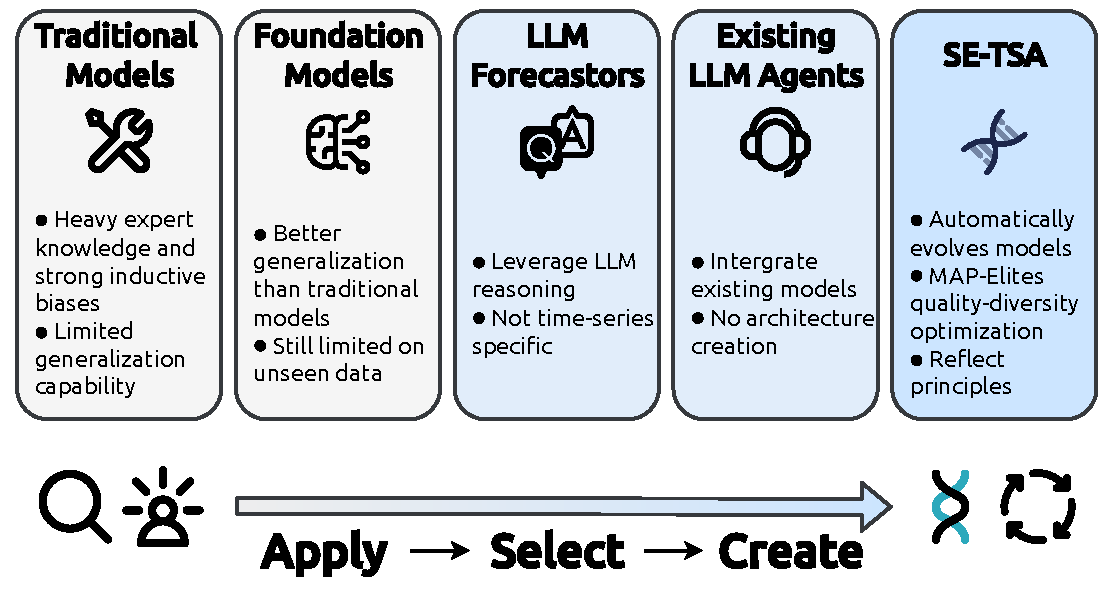
\includegraphics[width=\columnwidth]{figures/Comparison.pdf}
  \caption{Comparison between SE-TSA and existing time-series forecasting approaches.}
  \label{fig:comparison}
\end{figure}
\end{nolinenumbers}

We compare SE-TSA with other approaches as illustrated in Figure~\ref{fig:comparison}. The contributions of our proposed SE-TSA are summarized as follows:

\begin{enumerate}
  \item We propose SE-TSA, an LLM-driven evolution agent to create time-series forecasting architectures, which integrates an EXPLORE/EXPLOIT dual-strategy with MAP-Elites quality-diversity optimization.

  \item We introduce a reflection-based principle accumulation mechanism that enables interpretable meta-learning by summarizing architectural design principles in textual form.

  \item We conduct extensive experiments on nine cross-domain datasets against ten diverse baselines. Experimental results demonstrate that SE-TSA achieves superior performance on most datasets. Additional cross-domain transfer and ablation studies further validate the effectiveness of the proposed modules.
\end{enumerate}
\section{Related Work}

\subsection{Hand-Crafted Models and Foundation Models}

A large number of research has focused on manually designed architectures for time-series forecasting~\cite{CrossLinear,TimesNet,Duet,TimeXer}. For example, DUET~\cite{Duet} adpots dual clustering on the temporal and channel dimensions to enhance multivariate time series forecasting. PatchTST~\cite{PatchTST} divides time series into local patches and adopts a channel-independent processing strategy, achieving substantial loss reductions over standard Transformer baselines.% TimeXer~\cite{TimeXer} further introduces patch-wise and variate-wise attention mechanisms to better integrate endogenous and exogenous information.

Despite their strong empirical performance, these methods share an inherent limitation: their architectures are manually designed based on human assumptions, such as periodic decomposition patterns or inter-variable dependencies. As a result, their effectiveness may deteriorate when applied to datasets with substantially different distributions.% In addition, hand-crafted architecture design requires extensive domain expertise and iterative tuning. Once constructed, the resulting models remain static and can hardly adapt to new datasets without additional redesign and optimization.

Recent time-series foundation models trained on large-scale datasets, such as Sundial~\cite{Sundial}, Chronos~\cite{Chronos,Chronos2}, and TimesFM~\cite{TimesFM}, exhibit improved generalization ability and certain zero-shot forecasting capabilities. Nevertheless, they still encounter similar challenges when facing previously unseen datasets with distinct distributional properties.

\subsection{LLM-Based Forecasting Models and Agents}

Recent studies have explored incorporating LLMs into time-series forecasting by transforming numerical sequences into textual representations. For instance, Time-LLM~\cite{TimeLLM} introduces a reprogramming framework that adapts pretrained LLMs for forecasting tasks without modifying the backbone LLM. However, LLMs lack temporal inductive biases, thereby exhibit unstable performance across datasets.

More recently, agent-based systems have been proposed to automate the forecasting pipeline. TimeCopilot~\cite{TimeCopilot} integrates multiple time-series models with LLMs, enabling automated feature analysis, model selection, and forecast generation. TimeSeriesScientist~\cite{TimeSeriesScientist} proposes a multi-agent system composed of Curator, Planner, Forecaster, and Reporter agents, which collaboratively perform forecasting with report generation. Nevertheless, these agent systems primarily function as orchestration frameworks rather than architecture creation frameworks, which limits their adaptability and performance potential.

\subsection{Quality-Diversity Optimization}

QD optimization aims to generate diverse collections of high-performing solutions distributed across a predefined behavior regions. A representative example is MAP-Elites~\cite{MAP_Elites}, which maintains an archive of elite solutions over multi-dimensional regions, simultaneously preserving behavioral diversity and improving solution quality within each region. QD algorithms have been widely applied to neural architecture search~\cite{neural_architecture_search} and neuroevolution~\cite{neuroevolution}, where diversity preservation across architectural families helps mitigate convergence to local optima.
\section{Methodology}

\subsection{Problem Definition}

This paper focuses on time-series forecasting with exogenous variables. We adopt this setting for two reasons: first, it is widely encountered in real-world applications and is an important topic in academia~\cite{CrossLinear,TimeXer,DAG}; second, it forces the forecasting model to capture not only temporal dependencies but also variable dependencies, thereby providing a more challenging and representative evaluation setting.

Given a multivariate time series, each observation $\mathbf{x}_{t} \in \mathbb{R}^{F}$ at time $t$ contains both endogenous variable (forecasting target) and exogenous variables. Let the historical observation window be $\mathbf{X}_{t-L_{\text{in}}+1:t}  = (\mathbf{x}_{t-L_{\text{in}}+1},\mathbf{x}_{t-L_{\text{in}}+2},\dots,\mathbf{x}_{t}) \in \mathbb{R}^{L_{\text{in}} \times F}$. The forecasting objective is to learn a mapping:
\begin{equation}
\mathbf{\hat{X}}_{t+1:t+L_{\text{out}}}^{\text{endo}} = f_{\theta}\left(\mathbf{X}_{t-L_{\text{in}}+1:t}\right),
\end{equation}
where the goal is to predict the future $L_{\text{out}}$ steps of the endogenous variables based on a historical window of length $L_{\text{in}}$. In conventional forecasting frameworks, the architecture of $f_{\theta}$ is manually designed. In contrast, the proposed SE-TSA automatically creates the architecture topology through LLM-driven programmatic evolution.

\begin{nolinenumbers}
\begin{figure*}[htbp]
  \centering
  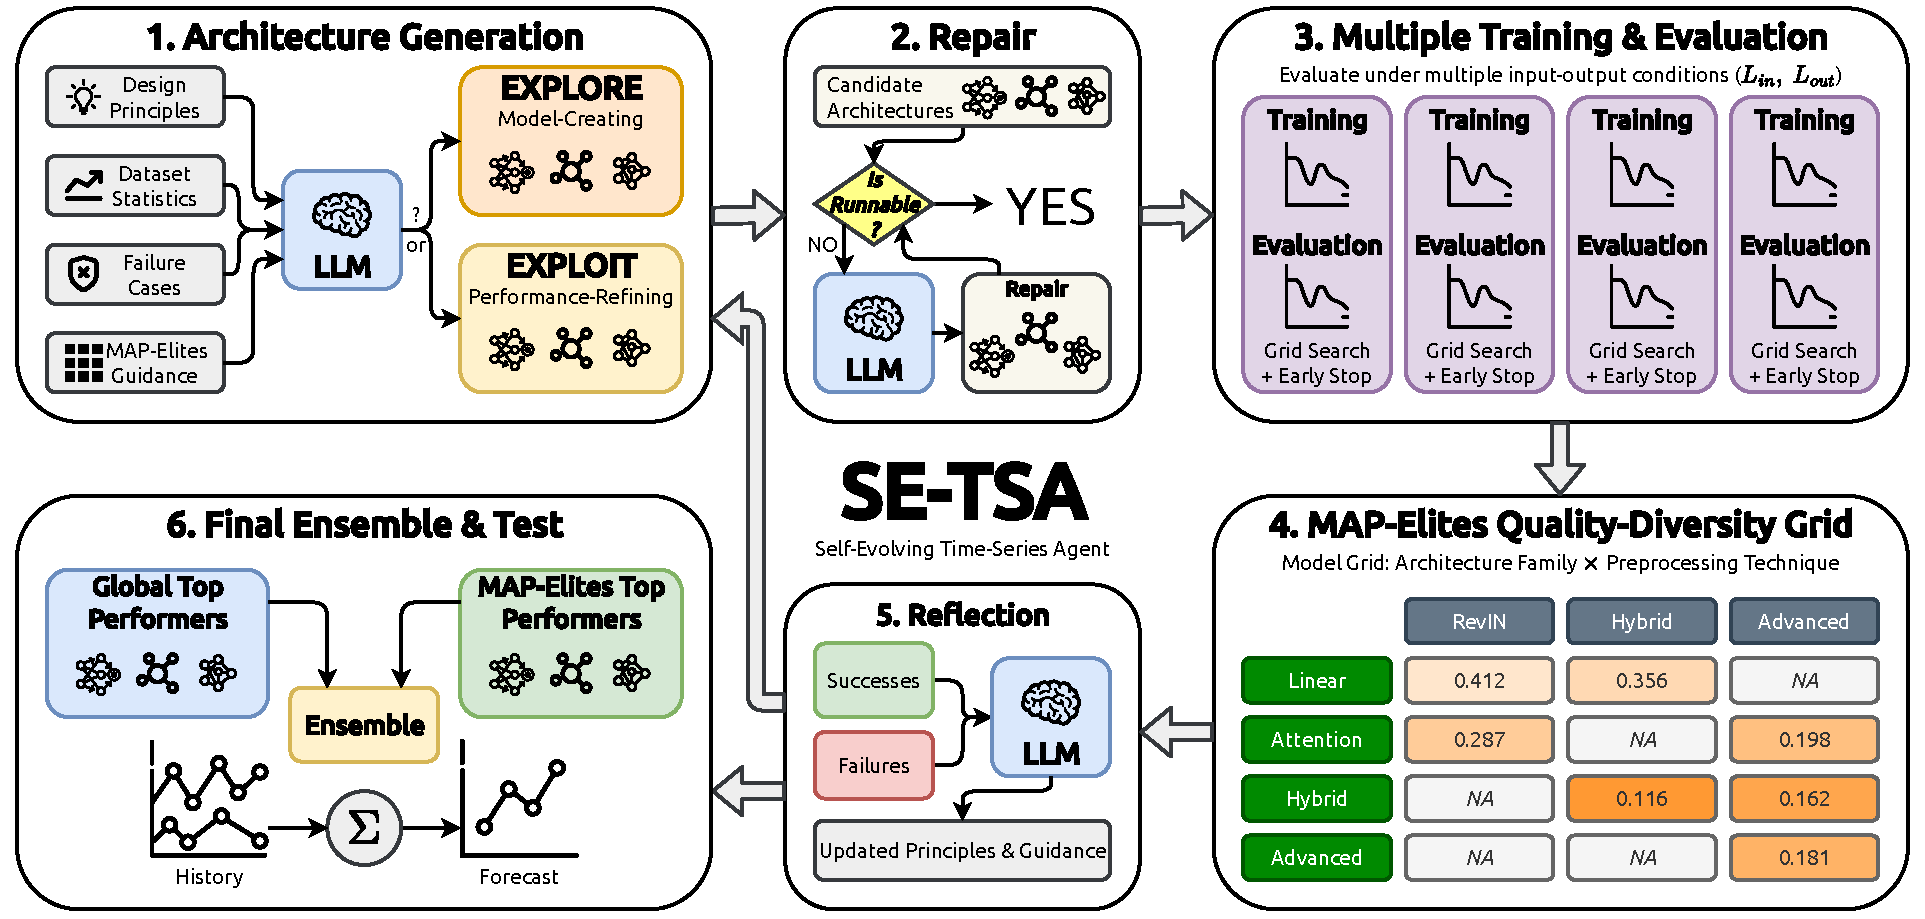
\includegraphics[width=0.98\textwidth]{figures/SE-TSA.pdf}
  \caption{Overall framework of SE-TSA. The agent system generates candidate architectures through EXPLORE/EXPLOIT dual strategies, updates the MAP-Elites quality-diversity grid after multi-condition evaluation, and accumulates interpretable design principles through a reflection mechanism, forming an iterative evolution loop.}
  \label{fig:framework}
\end{figure*}
\end{nolinenumbers}

\subsection{SE-TSA Overall Framework}

Figure~\ref{fig:framework} illustrates the overall framework of SE-TSA. Given a target dataset, SE-TSA iteratively executes the following pipeline within a predefined time budget:
\begin{enumerate}
  \item \textbf{Dual-strategy model creation}: The large language model dynamically selects either the EXPLORE strategy to create novel architectures, or the EXPLOIT strategy to refine existing high-performing architectures.

  \item \textbf{Multi-condition evaluation}: Each candidate will be validated for runnability; any non-runnable candidate will undergo a repair process. Runnable candidate models are trained and evaluated under all $(L_{\text{in}}, L_{\text{out}})$ settings. Hyperparameter search is first performed before full training.

  \item \textbf{MAP-Elites update}: Evaluated candidate models are assigned to corresponding cells in the quality-diversity grid according to their inferred architecture family and preprocessing strategy.

  \item \textbf{Reflection and principle accumulation}: After each iteration, the large language model analyzes the created models of the current round to extract design principles. Newly generated principles are deduplicated and incorporated into subsequent prompts, enabling cross-iteration meta-learning.
\end{enumerate}

After the evolutionary process terminates, representative models are selected from both the global history and the MAP-Elites archive to construct an ensemble for final forecasting.

All candidate models are trained by minimizing the mean squared error (MSE) loss between predictions and ground-truth target values:
\begin{equation}
\mathcal{L}_{\text{MSE}} = \frac{1}{T} \sum_{t=1}^{T} \left|\left| \mathbf{\hat{X}}_{t+1:t+L_{\text{out}}}^{\text{endo}} - \mathbf{X}_{t+1:t+L_{\text{out}}}^{\text{endo}} \right|\right|_{2},
\end{equation}
where $T$ denotes the number of training samples.

\subsection{Dual-Strategy Model Generation}

The model generation module is built upon an EXPLORE/EXPLOIT dual-strategy mechanism that dynamically balances architectural diversity and performance-oriented refinement. Before each iteration, the system probabilistically chooses between exploration and exploitation based on the MAP-Elites grid coverage ratio $c$ (see Section~\ref{method:map_elites}) and a decaying exploration rate $\varepsilon_t$:
\begin{equation}
p_{\text{explore}} = \max\left(\varepsilon_t, \frac{1-c}{K}\right),
\end{equation}
\begin{equation}
p_{\text{exploit}} = 1 - p_{\text{explore}},
\end{equation}
where $K$ controls the influence of grid coverage on strategy selection. The exploration rate follows an exponential decay schedule:
\begin{equation}
\varepsilon_t = \max\left(\varepsilon_{\min}, \varepsilon_{\text{base}} \cdot \gamma^t\right),
\end{equation}
where the default hyperparameters are $\varepsilon_{\text{base}}=0.9$, $\gamma=0.9$, and $\varepsilon_{\min}=0.1$. The complete generation prompts are provided in Appendix~\ref{app:prompts}.

\subsubsection{EXPLORE: Architecture Creation}

When the exploration strategy is selected, LLM is encouraged to create architectures to occupy previously unfilled regions in the MAP-Elites grid. Specifically, the system generates $N$ candidate models with diverse architectural patterns. The generation prompt incorporates four categories of information: (1) statistical summaries of the training dataset; (2) identifiers of currently unoccupied cells; (3) historically accumulated design principles; and (4) recent failure cases (e.g., unrunnable models).

By explicitly steering generation toward underexplored regions of MAP-Elite grid, the EXPLORE strategy expands the architectural diversity and improves coverage of the search space.

\subsubsection{EXPLOIT: Architecture Refinement}

When the exploitation strategy is selected, the agent system first groups models in the MAP-Elites grid according to architecture families. From each of the top-$k$ families, the model achieving the lowest loss on validation set is selected as the parent model. LLM then generates refined variants based on these information: (1) parent model specification; (2) second-best model within the same family; (3) globally best-performing model; (4) accumulated design principles; and (5) related failure cases.

Unlike EXPLORE, which emphasizes diversity expansion, the EXPLOIT strategy focuses on localized optimization while preserving the core mechanisms of validated architecture families. This enables performance refinement of occupied regions of MAP-Elite grid.

\subsection{Multi-Condition Evaluation}

Each generated candidate model first undergoes validation and automatic repair to ensure executability. Failure cases, together with their corresponding error information, are stored in a historical memory pool and used to guide future generation. Only executable candidate models proceed to the subsequent multi-condition evaluation stage.

The evaluation pipeline consists of two sequential phases:

\textbf{Configuration-space quick search}. To efficiently identify suitable hyperparameter settings, the agent system randomly samples at most $C$ candidate configurations and performs short-epoch training for each configuration. The configuration achieving the lowest validation loss is selected as the candidate configuration.

\textbf{Full training and validation}. Using the selected configuration, the candidate model is fully trained with the AdamW optimizer~\cite{AdamW} and MSE loss function.

Following the previous settings of the area~\cite{TimeMMD}, each candidate model is evaluated under multiple input--output conditions. The overall performance of a candidate model is defined as the average validation loss across all $(L_{\text{in}}, L_{\text{out}})$ conditions:
\begin{equation}
\bar{\mathcal{L}}_{\text{val}} = \frac{1}{|\mathcal{C}|}
\sum_{(L_{\text{in}}, L_{\text{out}})\in\mathcal{C}} \mathcal{L}_{\text{val}}^{(L_{\text{in}}, L_{\text{out}})},
\end{equation}
where $\mathcal{C}$ denotes the set of all input--output conditions, and $\mathcal{L}_{\text{val}}$ is MSE loss on validation set. A candidate model is allowed to replace the existing model within a MAP-Elites family only if its average validation loss $\bar{\mathcal{L}}_{\text{val}}$ is lower than that of the current one.

\subsection{MAP-Elites Quality-Diversity Grid}
\label{method:map_elites}

SE-TSA organizes evaluated candidate models within a two-dimensional MAP-Elites behavior space to jointly optimize model quality and architectural diversity. Each candidate is mapped to a behavioral region according to two discrete descriptors:

\textbf{Architecture family}: \textit{Linear}, \textit{Attention}, \textit{Hybrid}, and \textit{Advanced}, determined through code-level classification and analysis of the architectural pattern;

\textbf{Preprocessing family}: \textit{RevIN}~\cite{RevIN}, \textit{Hybrid}, and \textit{Advanced}, identified according to the employed normalization and preprocessing strategies.

The resulting behavior space contains $N_{\text{cells}} = 4 \times 3 = 12$ distinct cells. Each cell maintains the candidate model achieving the lowest validation loss within its corresponding behavioral region. Such a design, with limited expert knowledge, mitigates local optima in architectures and reduces overfitting on the validation set.

To quantify the exploration status of the search space, grid coverage is defined as the ratio between occupied cells and the total number of cells:
\begin{equation}
c = \frac{n_{\text{occupied}}}{N_{\text{cells}}},
\end{equation}
where $n_{\text{occupied}}$ denotes the number of currently populated cells.

The coverage ratio directly influences the EXPLORE/EXPLOIT decision mechanism. Specifically, low coverage increases the probability of selecting the EXPLORE strategy, encouraging the creation of architectures in underexplored behavioral regions. Conversely, high coverage shifts the search process toward EXPLOIT, allocating more computational resources to the refinement of high-performing architecture families.

\subsection{Reflection and Design Principle Accumulation}

The reflection mechanism serves as the core component enabling cross-iteration meta-learning in SE-TSA. After each iteration, the agent system identifies the best-performing and worst-performing models of the current round and constructs a reflection prompt containing complete evolutionary history, current MAP-Elites status, recent failure cases, and accumulated design principles. The complete reflection prompts are provided in Appendix~\ref{app:prompts}.

Based on this contextual information, LLM generates new design principles, which are interpretable high-level rules regarding architectural patterns, hyperparameter configurations, or preprocessing strategies.

To avoid redundant or semantically overlapping principles, each newly generated principle is encoded into a semantic embedding vector $\mathbf{p} \in \mathbb{R}^{d}$ using a BERT-like embedding model \texttt{all-MiniLM-L6-v2}~\cite{BERT,Sentence_BERT}. Cosine similarity is then computed against all previously stored principles:
\begin{equation}
\text{sim}(\mathbf{p}_{\text{new}}, \mathbf{p}_{\text{existing}}) = \frac{\mathbf{p}_{\text{new}} \cdot \mathbf{p}_{\text{existing}}}{\|\mathbf{p}_{\text{new}}\| \, \|\mathbf{p}_{\text{existing}}\|}.
\end{equation}

A newly generated principle is retained only if
\begin{equation}
\max_{\text{existing}} \text{sim}(\mathbf{p}_{\text{new}}, \mathbf{p}_{\text{existing}}) < \tau,
\end{equation}
where $\tau$ denotes the similarity threshold.

The accumulated design principles are subsequently injected into future prompts. This mechanism enables SE-TSA to progressively leverage cross-iteration induced domain knowledge during architecture creation, rather than relying solely on numerical information of data and architectures.

\subsection{Ensemble Prediction}

After the evolutionary process terminates, the final forecasting results are predicted through an ensemble module. Ensemble members are selected from two complementary candidate pools:

\textbf{Global-best pool}: the top-$N_1$ models with the lowest overall validation loss across the entire evolution process;

\textbf{Regional-best pool}: the top-$N_2$ elite models selected from different MAP-Elites behavioral regions.

Models appearing in both pools are retained with duplicated weights, thereby assigning greater influence to architectures that simultaneously achieve strong global performance and regional behavioral superiority.

Before inference, each selected ensemble member is retrained using the training set. The final prediction is then obtained through uniform averaging over all selected ensemble members:
\begin{equation}
\hat{\mathbf{X}}_{t+1:t+L_{\text{out}}}^{\text{ensemble}} =
\frac{1}{|\mathcal{M}|} \sum_{m \in \mathcal{M}} \hat{\mathbf{X}}_{t+1:t+L_{\text{out}}}^{(m)},
\end{equation}
where $\mathcal{M}$ denotes the set of all selected ensemble members.

By combining globally optimal models with behaviorally diverse elites, the ensemble strategy improves robustness and generalization ability while reducing the risk of overfitting to a single architecture family.

\begin{nolinenumbers}
\begin{table*}[htbp]
\centering
\caption{Main experimental results. Full results are in Appendix~\ref{app:main_results}. All values are average MAE and MAPE (\%) across all conditions. Red background: best result; blue background: second-best result.}
\label{tab:main_results}
\footnotesize
\setlength{\tabcolsep}{1.5pt}
\resizebox{\textwidth}{!}{%
\begin{tabular}{l | cc | cc | cc | cc | cc | cc | cc | cc | cc | cc | cc}
\toprule
& \multicolumn{2}{c|}{SE-TSA} & \multicolumn{2}{c|}{DLinear} & \multicolumn{2}{c|}{PatchTST} & \multicolumn{2}{c|}{TiDE} & \multicolumn{2}{c|}{TimeXer} & \multicolumn{2}{c|}{Kimi K2.6} & \multicolumn{2}{c|}{DeepSeek V4 Flash} & \multicolumn{2}{c|}{Gemma4 26B A4B} & \multicolumn{2}{c|}{Qwen3.6 35B A3B} & \multicolumn{2}{c|}{Moirai 2.0} & \multicolumn{2}{c}{TimeCopilot} \\
\cmidrule(lr){2-3} \cmidrule(lr){4-5} \cmidrule(lr){6-7} \cmidrule(lr){8-9} \cmidrule(lr){10-11} \cmidrule(lr){12-13} \cmidrule(lr){14-15} \cmidrule(lr){16-17} \cmidrule(lr){18-19} \cmidrule(lr){20-21} \cmidrule(lr){22-23}
Dataset & MAE & MAPE & MAE & MAPE & MAE & MAPE & MAE & MAPE & MAE & MAPE & MAE & MAPE & MAE & MAPE & MAE & MAPE & MAE & MAPE & MAE & MAPE & MAE & MAPE \\
\midrule
Agriculture & \best{5.97E+00} & \best{2.71} & 6.92E+00 & 3.12 & \second{6.06E+00} & \second{2.74} & 6.79E+00 & 3.04 & 6.60E+00 & 2.97 & 9.23E+00 & 4.18 & 8.24E+00 & 3.69 & 8.36E+00 & 3.72 & 7.31E+00 & 3.26 & 8.82E+00 & 3.98 & 9.20E+00 & 4.27 \\
Climate & \best{4.34E-01} & \best{17.88} & 4.98E-01 & 21.20 & \second{4.83E-01} & \second{19.95} & 5.06E-01 & 21.06 & 4.85E-01 & 20.08 & 5.40E-01 & 23.88 & 4.85E-01 & 20.75 & 4.97E-01 & 21.84 & 4.93E-01 & 21.21 & 5.50E-01 & 22.95 & 9.95E-01 & 40.77 \\
Economy & \best{8.27E+03} & \best{10.14} & 9.08E+03 & 11.56 & \second{8.67E+03} & \second{10.63} & 9.87E+03 & 12.26 & 9.21E+03 & 11.23 & 1.56E+04 & 18.44 & 1.61E+04 & 19.69 & 1.54E+04 & 18.15 & 1.48E+04 & 17.89 & 1.29E+04 & 15.82 & 1.09E+04 & 13.54 \\
Energy & \best{3.25E-01} & \best{10.07} & 4.06E-01 & 12.55 & 3.87E-01 & 11.95 & 3.80E-01 & 11.77 & 4.12E-01 & 12.74 & 5.04E-01 & 14.76 & 4.14E-01 & 12.16 & 4.13E-01 & 12.18 & 3.99E-01 & 11.94 & \second{3.49E-01} & \second{10.77} & 4.53E-01 & 14.43 \\
Environment & \best{2.10E+01} & \best{33.00} & 2.42E+01 & 37.29 & 2.39E+01 & 36.98 & 2.33E+01 & \second{33.96} & \second{2.30E+01} & 36.01 & NA & NA & NA & NA & NA & NA & NA & NA & 2.77E+01 & 41.91 & 2.93E+01 & 44.27 \\
PublicHealth & \best{9.80E-01} & \best{48.13} & 1.19E+00 & 64.64 & 1.54E+00 & 84.51 & 1.14E+00 & 56.20 & 1.53E+00 & 86.65 & 2.12E+00 & 118.30 & 1.25E+00 & 53.80 & 1.59E+00 & 73.73 & 1.36E+00 & 61.06 & \second{1.08E+00} & \second{48.90} & 1.85E+00 & 97.98 \\
Security & \best{1.63E+09} & 71.71 & 1.67E+09 & 73.75 & 1.78E+09 & 76.69 & 1.86E+09 & 80.81 & 1.70E+09 & 68.71 & 2.09E+09 & 78.06 & 1.81E+09 & 73.27 & 1.65E+09 & \best{66.54} & 1.74E+09 & \second{68.38} & \second{1.64E+09} & 73.06 & 1.71E+09 & 80.46 \\
SocialGood & \best{8.08E-01} & \best{12.83} & 8.30E-01 & 13.98 & 8.22E-01 & 13.61 & 8.57E-01 & 14.46 & \second{8.09E-01} & \second{13.44} & 1.28E+00 & 20.77 & 1.14E+00 & 17.92 & 1.23E+00 & 20.81 & 1.16E+00 & 17.44 & 8.78E-01 & 14.20 & 8.32E-01 & 13.59 \\
Traffic & \best{1.03E+04} & \best{4.31} & 1.66E+04 & 6.74 & \second{1.08E+04} & \second{4.49} & 1.61E+04 & 6.52 & 1.22E+04 & 5.03 & 2.60E+04 & 10.26 & 4.01E+04 & 15.62 & 2.92E+04 & 11.36 & 3.04E+04 & 11.95 & 2.38E+04 & 9.35 & 3.31E+04 & 12.99 \\
\bottomrule
\end{tabular}%
}
\end{table*}
\end{nolinenumbers}

\section{Experiments}

We adopt datasets compiled by Time-MMD~\cite{TimeMMD}, which include nine subsets from diverse domains, thereby enabling a comprehensive and fair comparison. Dataset descriptions and preprocessing details are provided in Appendix~\ref{app:implementation}. Forecasting performance is evaluated using two standard metrics, namely Mean Absolute Error (MAE) and Mean Absolute Percentage Error (MAPE):
\begin{equation}
\text{MAE} = \frac{1}{T} \sum_{t=1}^{T} \left\| \mathbf{\hat{X}}_{t+1:t+L_{\text{out}}}^{\text{endo}} - \mathbf{X}_{t+1:t+L_{\text{out}}}^{\text{endo}} \right\|,
\end{equation}
\begin{equation}
\text{MAPE} = \frac{100\%}{T} \sum_{t=1}^{T}
\frac
{\left\| \mathbf{\hat{X}}_{t+1:t+L_{\text{out}}}^{\text{endo}} - \mathbf{X}_{t+1:t+L_{\text{out}}}^{\text{endo}} \right\|}
{\left\| \mathbf{X}_{t+1:t+L_{\text{out}}}^{\text{endo}} \right\| },
\end{equation}
where $\mathbf{\hat{X}}_{t+1:t+L_{\text{out}}}^{\text{endo}}=\mathbf{\hat{X}}_{t+1:t+L_{\text{out}}}^{\text{ensemble}}$ and $\mathbf{X}_{t+1:t+L_{\text{out}}}^{\text{endo}}$ denote the predicted and ground-truth endogenous variables, respectively.

\subsection{Main Results}

Table~\ref{tab:main_results} summarizes the main experimental results across all benchmark datasets. The detailed result and benchmark settings can be found in Appendix~\ref{app:main_results}. SE-TSA and TimeCopilot use Kimi K2.6~\cite{Kimi} as LLM server.

Generally, SE-TSA achieves the best MAE performance on all nine datasets, demonstrating strong and consistent forecasting precision across diverse domains. For the MAPE metric, SE-TSA obtains the best results on eight datasets and underperforms Gemma4~\cite{Gemma} on the Security dataset ($71.71\%$ versus $66.54\%$).

It is worth noting that the absolute MAE values on some datasets are relatively large. This phenomenon primarily reflects the large numerical scale and strong non-stationarity of the original time series.

In contrast, direct LLM inference baselines consistently exhibit inferior performance. Moreover, smaller language models like Gemma4 26B A4B and Qwen3.6 35B A3B~\cite{Qwen} can outperform larger ones --- Kimi K2.6 and Deepseek V4~\cite{Deepseek} --- on certain datasets, suggesting that scaling model size alone does not effectively address time-series forecasting challenges.

Among the compared baselines, the time-series foundation model Moirai 2.0  and deep learning model PatchTST achieve competitive performance and attain the second-best results on several datasets. However, their performance remain inconsistent across different domains, whereas SE-TSA demonstrates substantially stronger robustness and generalization ability.

\begin{nolinenumbers}
\begin{table}[htbp]
\centering
\caption{Domain transfer results. Full results are in Appendix~\ref{app:domain_tranfer}. All values are average MAE and MAPE (\%) across all conditions. Red background: best result; blue background: second-best result.}
\label{tab:domain_transfer}
\small
\setlength{\tabcolsep}{2pt}
\resizebox{\columnwidth}{!}{%
\begin{tabular}{l | cc | cc | cc | cc | cc}
\toprule
\multicolumn{1}{r|}{Source} & \multicolumn{2}{c|}{Agriculture} & \multicolumn{2}{c|}{Climate} & \multicolumn{2}{c|}{Environment} & \multicolumn{2}{c|}{PublicHealth} & \multicolumn{2}{c}{Traffic} \\
\cmidrule(lr){2-3} \cmidrule(lr){4-5} \cmidrule(lr){6-7} \cmidrule(lr){8-9} \cmidrule(lr){10-11}
Target & MAE & MAPE & MAE & MAPE & MAE & MAPE & MAE & MAPE & MAE & MAPE \\
\midrule
Agriculture & \best{5.97E+00} & \best{2.71} & 1.19E+01 & 5.37 & 6.61E+00 & 2.97 & \second{6.00E+00} & \best{2.71} & 6.08E+00 & 2.75 \\
\midrule
Climate & 4.67E-01 & 19.37 & \best{4.34E-01} & \best{17.88} & \second{4.59E-01} & 19.12 & 4.66E-01 & 19.36 & 4.63E-01 & \second{19.04} \\
\midrule
Environment & 2.27E+01 & 34.92 & NA & NA & \best{2.10E+01} & \best{33.00} & \second{2.19E+01} & \best{33.00} & 2.24E+01 & 34.62 \\
\midrule
PublicHealth & \second{1.13E+00} & \second{54.74} & 7.86E+01 & 4363.87 & 1.18E+00 & 56.01 & \best{9.80E-01} & \best{48.13} & 1.20E+00 & 59.55 \\
\midrule
Traffic & \second{1.10E+04} & \second{4.59} & 1.48E+04 & 5.83 & 1.32E+04 & 5.48 & 1.14E+04 & 4.73 & \best{1.03E+04} & \best{4.31} \\
\bottomrule
\end{tabular}%
}
\end{table}
\end{nolinenumbers}

\subsection{Domain Transfer Analysis}

Table~\ref{tab:domain_transfer} presents the results of directly transferring the forecasting architectures obtained from one domain (dataset) to another domain.

Architectures evolved on a specific domain consistently achieve their best performance when evaluated on the same domain. For instance, the PublicHealth-evolved models achieve the best MAE of $0.980$ on PublicHealth, whereas transferring the Climate architectures to PublicHealth results in a dramatic degradation to $78.6$ MAE and $4363.87\%$ MAPE. Similarly, on the Traffic dataset, the in-domain architectures achieve an MAE of $1.03\times10^4$, outperforming transferred architectures by at least $6.4\%$.

These results indicate that the evolved architectures capture domain-specific characteristics. Therefore, SE-TSA does not merely identify generic forecasting structures, but instead automatically evolves architectures that are specialized for different datasets and domains.

\begin{nolinenumbers}
\begin{table}[htbp]
\centering
\caption{Ablation study results. Full results are in Appendix~\ref{app:ablation}. All values are average MAE and MAPE (\%) across all conditions. Red background: best result; blue background: second-best result.}
\label{tab:ablation}
\small
\setlength{\tabcolsep}{3pt}
\resizebox{\columnwidth}{!}{%
\begin{tabular}{l | cc | cc | cc | cc}
\toprule
& \multicolumn{2}{c|}{w/o Reflection} & \multicolumn{2}{c|}{w/o MAP-Elites} & \multicolumn{2}{c|}{w/o Ensemble} & \multicolumn{2}{c}{SE-TSA} \\
\cmidrule(lr){2-3} \cmidrule(lr){4-5} \cmidrule(lr){6-7} \cmidrule(lr){8-9}
Dataset & MAE & MAPE & MAE & MAPE & MAE & MAPE & MAE & MAPE \\
\midrule
Agriculture & \second{6.15E+00} & \second{2.76} & 6.67E+00 & 2.99 & 6.43E+00 & 2.90 & \best{5.97E+00} & \best{2.71} \\
Climate & \second{4.35E-01} & \second{18.00} & 4.52E-01 & 18.60 & 4.54E-01 & 18.60 & \best{4.34E-01} & \best{17.88} \\
Environment & \second{2.11E+01} & 33.13 & 2.12E+01 & \second{33.05} & 2.18E+01 & 34.45 & \best{2.10E+01} & \best{33.00} \\
PublicHealth & 1.06E+00 & 51.77 & \second{9.84E-01} & \best{47.81} & 9.91E-01 & 49.08 & \best{9.80E-01} & \second{48.13} \\
Traffic & 1.11E+04 & 4.63 & \second{1.05E+04} & 4.39 & \second{1.05E+04} & \second{4.37} & \best{1.03E+04} & \best{4.31} \\
\bottomrule
\end{tabular}%
}
\end{table}
\end{nolinenumbers}

\subsection{Ablation Study}

Table~\ref{tab:ablation} shows the result of ablation study by removing MAP-Elites (coupled with dual-strategy model generation), reflection, and ensemble.

In most cases, removing any module leads to increased MAE and MAPE, demonstrating the effectiveness of the complete agent system design. The extent of performance degradation differs across datasets, suggesting that different domains benefit from different modules of SE-TSA. For example, removing MAP-Elites (which also removes the difference between EXPLORE and EXPLOIT) causes the most significant percentage degradation of MAPE on Agriculture (MAPE from $2.71$ to $2.99$, with $10.3\%$ degradation). In contrast, removing MAP-Elites has little effect on PublicHealth, where the performance remains close to that of the full agent system. Despite these domain-specific differences, the complete SE-TSA consistently achieves the best or near-best performance across all datasets, demonstrating that the proposed modules can complement each other and jointly improve the effectiveness of SE-TSA.

\begin{nolinenumbers}
\begin{table}[htbp]
\centering
\caption{Representative design principles extracted during evolution.}
\label{tab:principles_by_domain}
\small
\setlength{\tabcolsep}{2pt}
\begin{tabular}{l>{\raggedright\arraybackslash}p{1.2cm}>{\raggedright\arraybackslash}p{4.5cm}}
\toprule
\textbf{Dataset} & \textbf{Attribute} & \textbf{Representative Principle} \\
\midrule
Climate & Short seq, small & Shallow ODE networks outperform deeper configurations on climate forecasting; continuous-time modeling benefits from simple dynamics functions rather than expressive ODE solvers. \\
\midrule
Security & Short seq, small, irregular & Small linear models outperform attention-based and hybrid architectures by 10--100$\times$. \\
\midrule
Environment & Long seq, 41 features, periodic & Multi-scale wavelet decomposition outperforms neural basis expansion. \\
\midrule
PublicHealth & Medium seq, 44 features, periodic & Real-valued FFT projections enable effective attention mechanisms on small datasets. \\
\midrule
Traffic & Short seq, 17 features, small & Cross-channel attention mechanisms catastrophically fail on small traffic datasets, performing 6$\times$ worse than channel-independent models. \\
\bottomrule
\end{tabular}
\end{table}
\end{nolinenumbers}

\subsection{Case Study}

Table~\ref{tab:principles_by_domain} lists the most representative principle from each dataset, selected to highlight how the evolved knowledge directly reflects the data's intrinsic properties. More case analysis can be found in Appendix~\ref{app:case_study}.

\subsubsection{Dataset Characteristics and Design Principles}

The principles reveal a direct correspondence between data characteristics and architectural choices. Small dataset (Climate) favor compact continuous-time models, whereas long-horizon, high-dimensional data (Environment) require multi-scale wavelet decomposition. Small-sample irregular data (Security) tend to converge toward simple linear models, while periodic multi-feature data (PublicHealth) benefit from real-valued frequency-domain preprocessing to facilitate attention mechanisms. Besides, small-sample traffic data (Traffic) exhibit catastrophic degradation under cross-channel interaction modeling. These observations suggest that the reflection mechanism adapts to the underlying data structure.

\subsubsection{Cross-Domain Principle Contrast}

We observe that similar design principles can lead to opposite outcomes depending on domain characteristics. For instance, feature interaction modeling fails dramatically on small low-dimensional datasets such as Traffic, yet becomes effective on high-dimensional datasets like PublicHealth when combined with appropriate preprocessing.

Moreover, simple linear models outperform attention-based architectures on small irregular datasets such as Security, whereas deep multi-scale decomposition is crucial for long-horizon high-dimensional datasets like Environment. These findings suggest that the appropriate level of model complexity should align with the underlying data distribution and structural properties of the dataset.

\begin{nolinenumbers}
\begin{figure}[htbp]
  \centering
  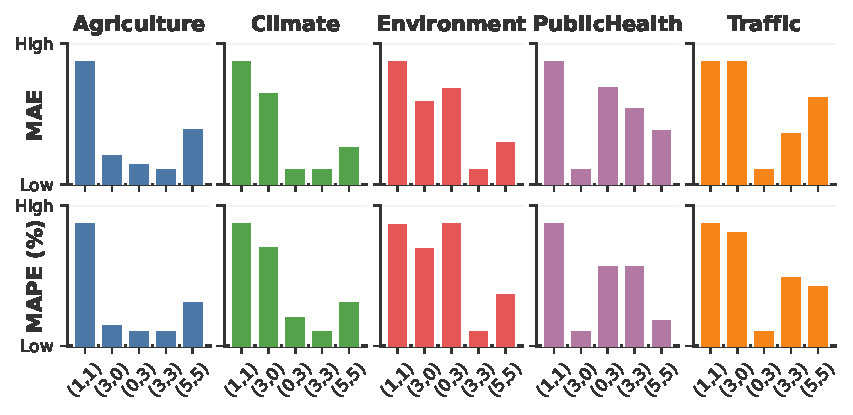
\includegraphics[width=\columnwidth]{figures/Hyperparam.pdf}
  \caption{Hyperparameter analysis of ensemble. Full results are in Appendix~\ref{app:hyperparam}.}
  \label{fig:hyperparam}
\end{figure}
\end{nolinenumbers}

\subsection{Hyperparameter Analysis of Ensemble Configuration}

The forecasting performance of SE-TSA is influenced by the ensemble module. To analyze its sensitivity, we evaluate five different $(N_{1}, N_{2})$ configurations: $(1,1)$, $(3,0)$, $(0,3)$, $(3,3)$, and $(5,5)$, where $(3,3)$ is the default setting.

As shown in Figure~\ref{fig:hyperparam}, the default $(3,3)$ achieves the superior performance on most datasets. In contrast, the single-source configurations ($(3,0)$ and $(0,3)$) yield inferior results. These observations indicate the effectiveness of jointly leveraging globally optimal models and behaviorally diverse elites. Although $(5,5)$ further increases the ensemble size, its performance does not improve consistently, likely because the additional models are relatively low-quality candidates.
\section{Conclusion}
This paper proposes SE-TSA, an agent system that automatically creates time-series forecasting architectures through LLM-driven programmatic evolution. Unlike prior agent systems that operate within predefined model libraries, SE-TSA iteratively creates and refines forecasting models through an EXPLORE/EXPLOIT dual-strategy optimization loop. The MAP-Elites quality-diversity mechanism mitigates premature convergence, while the reflection module progressively accumulates interpretable principles.

Experiments on nine cross-domain datasets show that SE-TSA achieves the best or the near-best results, generally outperforming diverse baseline methods. Domain-transfer experiments further validate the domain specificity of the evolved architectures. Ablation studies show that the reflection mechanism, MAP-Elites diversity maintenance, and Bagging ensemble each contribute measurably to the final forecasting performance.

\section*{Limitations}

Despite promising results, several limitations remain. First, due to budget constraints, several hyperparameters were set empirically without a comprehensive analysis. Second, the MAP-Elites behavior space (currently based only on architecture family and preprocessing type) could be refined. Third, the training pipeline applies a uniform strategy to all candidate models, whereas different model families may benefit from specialized procedures like warm-up for attention-based models. Finally, although SE-TSA uses a many-to-one evaluation paradigm, evolved architectures on some datasets still adopt channel-independent strategies, indicating that effective channel-wise modeling remains challenging.


\bibliography{custom}

\clearpage
\appendix
\section{Implementation Details and Hyperparameters}
\label{app:implementation}

\subsection{Datasets and Preprocessing}

Table~\ref{tab:datasets} summarizes the 9 datasets used in the experiments. All are multivariate time series with exogenous variables. Feature counts reflect post-preprocessing dimensions (including SVD-encoded text features). Feature counts vary widely, from $17$ (Traffic) to $44$ (PublicHealth), reflecting the differing amounts of exogenous information available in each domain. Long-horizon forecasting tasks use larger input and output windows --- up to $(96, 336)$ --- whereas short-horizon tasks use $(8, 12)$ at maximum.

\begin{nolinenumbers}
\begin{table}[htbp]
\caption{Dataset statistics. Feature counts are post-preprocessing.}
\label{tab:datasets}
\centering
\small
\setlength{\tabcolsep}{3pt}
\resizebox{\columnwidth}{!}{%
\begin{tabular}{lccc}
\toprule
Dataset & Features & Time steps & Input/Output \\
\midrule
Agriculture & 28 & 496 & (8,6), (8,8), (8,10), (8,12) \\
Climate & 29 & 496 & (8,6), (8,8), (8,10), (8,12) \\
Economy & 29 & 423 & (8,6), (8,8), (8,10), (8,12) \\
Energy & 24 & 2,105 & (36,12), (36,24), (36,36), (36,48) \\
Environment & 41 & 11,102 & (96,48), (96,96), (96,192), (96,336) \\
PublicHealth & 44 & 1,825 & (36,12), (36,24), (36,36), (36,48) \\
Security & 26 & 297 & (8,6), (8,8), (8,10), (8,12) \\
SocialGood & 26 & 900 & (8,6), (8,8), (8,10), (8,12) \\
Traffic & 17 & 945 & (8,6), (8,8), (8,10), (8,12) \\
\bottomrule
\end{tabular}%
}
\end{table}
\end{nolinenumbers}

The preprocessing pipeline proceeds as follows:

\textbf{Step 1: temporal indexing.} The loader searches for a \texttt{date} column, and converts it to \texttt{datetime}. The data are then sorted in ascending chronological order.

\textbf{Step 2: auxiliary timestamp conversion.} Any time columns (\texttt{start\_date}, \texttt{end\_date}, or \texttt{Month}) are converted to numeric values so that they can be fed into the model as regular regressors.

\textbf{Step 3: target-column reordering.} The target variable column \texttt{OT} is moved to the first position so that all evaluation metrics (MSE, MAE, MAPE) consistently operate on this column.

\textbf{Step 4: missing-value imputation.} Columns that are entirely empty are dropped. Remaining missing values are filled in two stages: forward fill and zero fill.

\textbf{Step 5: chronological split.} The time series is divided into training ($70\%$), validation ($10\%$), and test ($20\%$) sets in temporal order.

\textbf{Step 6: text-feature encoding.} All textual columns are encoded by the pre-trained BERT-like embedding model \texttt{all-MiniLM-L6-v2}, producing a $384$-dimensional semantic embedding for every row. Truncated SVD is then applied to reduce the embedding to \texttt{svd\_n\_components} dimensions (default $3$). The parameter of SVD is obtained on training set.

\textbf{Step 7: training-set statistics.} On the training split, these statistics are computed: sample count, feature count, per-feature mean/standard-deviation/min/max, trend strength (Pearson correlation between each feature and the time index), and the dominant period of the target column (via FFT). These statistics are fed into the LLM generation prompts as dataset context.

\textbf{Step 8: sliding-window construction.} For each $(L_{\text{in}}, L_{\text{out}})$ condition, samples are generated with a sliding window.

\begin{nolinenumbers}
\begin{table}[htbp]
\caption{Complete hyperparameter configuration of SE-TSA. Unless otherwise specified, all experiments use the same settings.}
\label{tab:hyperparams}
\centering
\small
\begin{tabular}{ll}
\toprule
Hyperparameter & Value \\
\midrule
Time budget & 360 minutes \\
Maximum iterations & 10 \\
Candidates per iteration (EXPLORE) & 5 \\
Exploitation top-$k$ families & 3 \\
Repair retry attempts & 2 \\
Initial exploration rate $\varepsilon_{\text{base}}$ & 0.9 \\
Exploration rate decay $\gamma$ & 0.9 \\
Minimum exploration rate $\varepsilon_{\text{min}}$ & 0.1 \\
Batch size & 32 \\
Learning rate & 0.001 \\
Maximum training epochs & 10 \\
Early stopping patience & 3 \\
Quick search max epochs & 3 \\
Quick search max combinations & 8 \\
Quick search max time & 10 minutes \\
Ensemble top-$N_1$ (global) & 3 \\
Ensemble top-$N_2$ (MAP-Elites) & 3 \\
Maximum principles & 5 \\
Principle similarity threshold & 0.7 \\
LLM max tokens & 196,608 \\
LLM retry attempts & 3 \\
\bottomrule
\end{tabular}
\end{table}
\end{nolinenumbers}

\subsection{Hyperparameters}

Table~\ref{tab:hyperparams} lists the complete hyperparameter configuration used for all experiments unless otherwise stated. The 360-minute time budget and the 10-iteration cap jointly constrain the total search cost, ensuring that SE-TSA remains computationally tractable. Besides, the quick-search limits (max epochs, max combinations, max time) prevent any single candidate architecture from consuming a disproportionate fraction of the iteration budget.

\section{LLM Prompts}
\label{app:prompts}

The following prompts illustrate the structure used in each stage of the SE-TSA pipeline. Variables denoted by \texttt{\$variable} are filled at runtime. All code-generation prompts share the same base rules (inheritance contract, shape requirements, normalization guidance).

\DefineVerbatimEnvironment{promptbox}{Verbatim}{fontsize=\scriptsize,frame=single,framesep=2mm,breaklines=true,breakanywhere=true}

\subsection{EXPLORE Prompt}

\begin{promptbox}
You are an expert deep-learning researcher specializing in time-series forecasting.
Your task is to generate PyTorch model code that inherits from `BaseForecastModel`.

## CRITICAL RULES (excerpt)
1. `forward()` MUST return shape `(batch_size, output_len, n_features)`.
2. Only use `torch` and standard Python libraries. No `numpy`.
3. Do NOT write training loops, data loading, or main blocks.
4. You MUST define `get_all_configs()` for tunable hyper-parameters.
5. Your ENTIRE response must be ONLY a single valid JSON object.
... (interface contract, parameter range guidance, RevIN reference,
 correct example, common mistakes, and shape annotation rules)

## Strategy: EXPLORE
Your goal is to generate NOVEL and DIVERSE architectures. Do not reuse existing
designs. Actively explore architecture families or novel combinations that have
not been tried yet. Be bold in trying new ideas.

## Task: Model Generation Request
Iteration: $iteration
Dataset Statistics: $data_stats
Empty MAP-Elites Cells: $empty_cells
Validated Design Principles: $principles
Recent Failures to Avoid: $failures

Generate $n_models diverse model designs for this dataset...
Return JSON: {"models": [{"class_name": ..., "code": ..., ...}]}
\end{promptbox}

\subsection{EXPLOIT Prompt}

\begin{promptbox}
You are an expert deep-learning researcher specializing in time-series forecasting.
Your task is to generate PyTorch model code that inherits from `BaseForecastModel`.

## CRITICAL RULES (excerpt)
... (same base rules as EXPLORE)

## Strategy: EXPLOIT
Your goal is to carefully improve the parent model while preserving its core
mechanism. Make targeted, evidence-based modifications. Do not change the
fundamental architecture family. Do NOT use comparative language like
"better than parent".

## Task: Model Improvement Request
Iteration: $iteration
Dataset Statistics: $data_stats
Parent Model: $parent_class_name (val_loss=$parent_val_loss,
 params=$parent_num_params, arch=$parent_arch_family)
Top Models in Same Family: $same_family_models
Global Best Model: $global_best_model
Recent Failed Variants: $failed_variants
Validated Design Principles: $principles

Generate ONE improved variant of the parent model...
Return JSON: {"models": [{"class_name": ..., "code": ..., ...}]}
\end{promptbox}

\subsection{REPAIR Prompt}

\begin{promptbox}
You are an expert deep-learning researcher specializing in time-series forecasting.
Your task is to generate PyTorch model code that inherits from `BaseForecastModel`.

## CRITICAL RULES (excerpt)
... (same base rules as EXPLORE)

## Strategy: REPAIR
Your goal is to make the MINIMAL change to fix the error while preserving the
original design intent. Do not rewrite the entire model. Keep the EXACT same
class name. Focus only on fixing the specific error shown.

## Task: Error Correction Request
Model: $class_name
Original Description: $description
Original Design Rationale: $design_rationale
Evaluation Error: $error_message
Broken Model Code: $code
Prior Failed Fix Attempts: $prior_attempts

Fix the error in the model code. The fixed model MUST preserve the original
architecture family and design intent...
Return JSON: {"models": [{"class_name": "$class_name", "code": ..., ...}]}
\end{promptbox}

\subsection{REFLECT Prompt}

\begin{promptbox}
You are an expert ML researcher. Provide concise, actionable insights.

## Task: Reflection Request
Iteration: $iteration
Best Model This Round: $best_model
Worst Model This Round: $worst_model
All Models This Round: $all_models
History Summary (last $history_rounds rounds): $history_summary
MAP-Elites Coverage: $coverage
Failures This Round: $failures
Existing Principles: $existing_principles

Analyze the results and identify the SINGLE most valuable new design principle.
Return exactly 1 principle that is NOT already in the existing principles above.
Return JSON: {"principles": ["principle"]}
\end{promptbox}

\section{Architecture Example}
\label{app:case_study}

This section presents the best-evolved model (\texttt{KoopmanAutoencoderForecast}) on the Climate dataset.

\subsection*{Why this design fits Climate data}

The Climate dataset exhibits short input sequences with 29 meteorological features. The learned design principles indicate that ``Koopman operator learning with compact latent spaces outperforms both high-dimensional Koopman variants and continuous-time neural networks on climate forecasting,'' and that ``continuous-time modeling benefits from simple dynamics functions rather than expressive ODE solvers.'' These principles align well with the statistical characteristic of the dataset. The source code is as below:

\begin{nolinenumbers}
\begin{promptbox}
import torch
import torch.nn as nn
from src.models.base import BaseForecastModel
from src.models.layers.revin import RevIN

class KoopmanAutoencoderForecast(BaseForecastModel):
    def __init__(self, input_len, output_len, n_features, config=None):
        super().__init__(input_len, output_len, n_features, config)
        self.latent_dim = self.config.get('latent_dim', 256)
        self.encoder_depth = self.config.get('encoder_depth', 3)
        self.n_koopman_blocks = self.config.get('n_koopman_blocks', 8)
        self.dropout_rate = self.config.get('dropout', 0.0)

        self.revin = RevIN(self.n_features, affine=True)

        # Encoder: (batch, input_len, n_features) -> (batch, latent_dim)
        encoder_layers = []
        in_dim = self.input_len * self.n_features
        for i in range(self.encoder_depth):
            out_dim = self.latent_dim if i == self.encoder_depth - 1 \\
                      else max(self.latent_dim, in_dim // 2)
            encoder_layers.append(nn.Linear(in_dim, out_dim))
            if i < self.encoder_depth - 1:
                encoder_layers += [nn.LayerNorm(out_dim), nn.GELU(), \\
                                   nn.Dropout(self.dropout_rate)]
            in_dim = out_dim
        self.encoder = nn.Sequential(*encoder_layers)

        # Koopman operator: block-diagonal for stability
        self.koopman_blocks = nn.ParameterList([
            nn.Parameter(torch.randn(
                self.latent_dim // self.n_koopman_blocks,
                self.latent_dim // self.n_koopman_blocks) * 0.01)
            for _ in range(self.n_koopman_blocks)])
        self.koopman_identity = nn.Parameter(
            torch.eye(self.latent_dim // self.n_koopman_blocks),
            requires_grad=False)

        # Decoder: (batch, latent_dim) -> (batch, output_len, n_features)
        decoder_layers = []
        in_dim = self.latent_dim
        for i in range(self.encoder_depth):
            out_dim = self.output_len * self.n_features if i == last \\
                      else max(self.latent_dim, in_dim // 2)
            decoder_layers.append(nn.Linear(in_dim, out_dim))
            if i < self.encoder_depth - 1:
                decoder_layers += [nn.LayerNorm(out_dim), nn.GELU(), \\
                                   nn.Dropout(self.dropout_rate)]
            in_dim = out_dim
        self.decoder = nn.Sequential(*decoder_layers)

    def apply_koopman(self, z, n_steps):
        block_size = self.latent_dim // self.n_koopman_blocks
        z_blocks = torch.split(z, block_size, dim=-1)
        results = []
        for zb, K in zip(z_blocks, self.koopman_blocks):
            K_eff = K + self.koopman_identity
            z_evolved = zb
            for _ in range(n_steps):
                z_evolved = torch.matmul(z_evolved, K_eff.T)
            results.append(z_evolved)
        return torch.cat(results, dim=-1)

    def forward(self, x):
        x = self.revin(x, mode='norm')
        x_flat = x.view(-1, self.input_len * self.n_features)
        z = self.encoder(x_flat)

        # Predict each step via Koopman evolution in latent space
        z_steps = []
        for t in range(1, self.output_len + 1):
            z_steps.append(self.apply_koopman(z, t))
        z_traj = torch.stack(z_steps, dim=1)

        z_traj_flat = z_traj.view(-1, self.latent_dim)
        out_flat = self.decoder(z_traj_flat)
        out = out_flat.view(-1, self.output_len, self.output_len, \\
                            self.n_features)
        out = torch.stack([out[:, i, i, :] \\
                           for i in range(self.output_len)], dim=1)

        out = self.revin(out, mode='denorm')
        return out
\end{promptbox}
\end{nolinenumbers}

The evolved architecture directly reflects these principles: it employs a Koopman operator --- which learns linear dynamics in a compact latent space --- rather than complex ODE solvers. The block-diagonal structure of the Koopman operator ensures stable evolution. The encoder and decoder use moderate depth (3 layers) with layer normalization and GELU activations, providing sufficient capacity without overfitting.

\begin{nolinenumbers}
\begin{table*}[htbp]
\centering
\caption{Full main results. Moirai 2.0 (ZS) and Moirai 2.0 (FT) report zero-shot and fine-tuned results, respectively. Red background: best result; blue background: second-best result.}
\label{tab:main_results_full}
\footnotesize
\setlength{\tabcolsep}{0.5pt}
\resizebox{\textwidth}{!}{%
\begin{tabular}{lc | cc | cc | cc | cc | cc | cc | cc | cc | cc | cc | cc | cc}
\toprule
& & \multicolumn{2}{c|}{SE-TSA} & \multicolumn{2}{c|}{DLinear} & \multicolumn{2}{c|}{PatchTST} & \multicolumn{2}{c|}{TiDE} & \multicolumn{2}{c|}{TimeXer} & \multicolumn{2}{c|}{Kimi K2.6} & \multicolumn{2}{c|}{DeepSeek V4 Flash} & \multicolumn{2}{c|}{Gemma4 26B A4B} & \multicolumn{2}{c|}{Qwen3.6 35B A3B} & \multicolumn{2}{c|}{Moirai 2.0 (ZS)} & \multicolumn{2}{c|}{Moirai 2.0 (FT)} & \multicolumn{2}{c}{TimeCopilot} \\
\cmidrule(lr){3-4} \cmidrule(lr){5-6} \cmidrule(lr){7-8} \cmidrule(lr){9-10} \cmidrule(lr){11-12} \cmidrule(lr){13-14} \cmidrule(lr){15-16} \cmidrule(lr){17-18} \cmidrule(lr){19-20} \cmidrule(lr){21-22} \cmidrule(lr){23-24} \cmidrule(lr){25-26}
Dataset & $L_{\text{out}}$ & MAE & MAPE & MAE & MAPE & MAE & MAPE & MAE & MAPE & MAE & MAPE & MAE & MAPE & MAE & MAPE & MAE & MAPE & MAE & MAPE & MAE & MAPE & MAE & MAPE & MAE & MAPE \\
\midrule
Agriculture&6&5.08E+00 & 2.31 & 5.98E+00 & 2.70 & \second{5.03E+00} & \second{2.28} & 5.79E+00 & 2.61 & \best{4.73E+00} & \best{2.18} & 6.35E+00 & 3.00 & 5.94E+00 & 2.76 & 5.90E+00 & 2.70 & 5.36E+00 & 2.46 & 6.19E+00 & 2.82 & 6.17E+00 & 2.81 & 6.84E+00 & 3.19 \\
&8&\best{5.68E+00} & \best{2.57} & 6.54E+00 & 2.95 & \second{6.00E+00} & \second{2.70} & 6.38E+00 & 2.87 & 6.39E+00 & 2.87 & 8.74E+00 & 3.96 & 7.88E+00 & 3.52 & 8.49E+00 & 3.75 & 6.89E+00 & 3.06 & 7.71E+00 & 3.50 & 7.72E+00 & 3.50 & 8.57E+00 & 3.97 \\
&10&\best{6.28E+00} & \second{2.87} & 7.20E+00 & 3.26 & \second{6.34E+00} & \best{2.86} & 7.02E+00 & 3.14 & 8.05E+00 & 3.60 & 1.15E+01 & 5.14 & 1.07E+01 & 4.73 & 9.67E+00 & 4.25 & 9.63E+00 & 4.23 & 9.77E+00 & 4.41 & 9.73E+00 & 4.39 & 1.00E+01 & 4.65 \\
&12&\best{6.87E+00} & \best{3.09} & 7.96E+00 & 3.56 & \second{6.88E+00} & \second{3.10} & 7.96E+00 & 3.55 & 7.23E+00 & 3.24 & 1.03E+01 & 4.65 & 8.42E+00 & 3.76 & 9.40E+00 & 4.19 & 7.36E+00 & 3.29 & 1.16E+01 & 5.21 & 1.14E+01 & 5.13 & 1.14E+01 & 5.27 \\
&Avg&\best{5.97E+00} & \best{2.71} & 6.92E+00 & 3.12 & \second{6.06E+00} & \second{2.74} & 6.79E+00 & 3.04 & 6.60E+00 & 2.97 & 9.23E+00 & 4.18 & 8.24E+00 & 3.69 & 8.36E+00 & 3.72 & 7.31E+00 & 3.26 & 8.82E+00 & 3.98 & 8.75E+00 & 3.96 & 9.20E+00 & 4.27 \\
\midrule
Climate&6&\best{4.37E-01} & \best{18.15} & 5.05E-01 & 21.81 & 4.86E-01 & 20.27 & 5.15E-01 & 21.64 & 4.95E-01 & 20.72 & 5.54E-01 & 24.42 & 5.18E-01 & 21.90 & 5.20E-01 & 22.39 & \second{4.75E-01} & \second{19.81} & 5.58E-01 & 23.56 & 5.72E-01 & 24.50 & 8.73E-01 & 36.55 \\
&8&\second{4.32E-01} & \second{17.70} & 4.96E-01 & 20.75 & 4.85E-01 & 20.04 & 5.08E-01 & 21.06 & 4.87E-01 & 19.92 & 4.79E-01 & 20.97 & \best{4.23E-01} & \best{17.60} & 4.86E-01 & 21.13 & 4.58E-01 & 19.67 & 5.57E-01 & 23.42 & 5.60E-01 & 23.63 & 9.63E-01 & 39.92 \\
&10&\best{4.33E-01} & \best{17.75} & 4.93E-01 & 20.97 & 4.76E-01 & \second{19.70} & 5.07E-01 & 21.02 & 4.86E-01 & 20.09 & 5.50E-01 & 24.54 & 4.61E-01 & 20.50 & \second{4.60E-01} & 20.87 & 5.01E-01 & 21.56 & 5.46E-01 & 22.69 & 5.59E-01 & 23.44 & 1.04E+00 & 42.12 \\
&12&\best{4.35E-01} & \best{17.91} & 4.97E-01 & 21.27 & 4.85E-01 & 19.80 & 4.95E-01 & 20.52 & \second{4.74E-01} & \second{19.60} & 5.77E-01 & 25.61 & 5.38E-01 & 23.02 & 5.20E-01 & 22.96 & 5.39E-01 & 23.81 & 5.37E-01 & 22.13 & 5.50E-01 & 22.94 & 1.11E+00 & 44.50 \\
&Avg&\best{4.34E-01} & \best{17.88} & 4.98E-01 & 21.20 & \second{4.83E-01} & \second{19.95} & 5.06E-01 & 21.06 & 4.85E-01 & 20.08 & 5.40E-01 & 23.88 & 4.85E-01 & 20.75 & 4.97E-01 & 21.84 & 4.93E-01 & 21.21 & 5.50E-01 & 22.95 & 5.60E-01 & 23.63 & 9.95E-01 & 40.77 \\
\midrule
Economy&6&\best{7.64E+03} & \best{9.37} & 8.58E+03 & 11.07 & \second{8.01E+03} & \second{9.89} & 9.52E+03 & 12.00 & 8.32E+03 & 10.16 & 1.13E+04 & 13.44 & 1.10E+04 & 13.89 & 1.09E+04 & 13.32 & 1.25E+04 & 15.74 & 1.25E+04 & 15.58 & 1.20E+04 & 14.97 & 1.04E+04 & 13.17 \\
&8&\best{7.93E+03} & \best{9.73} & 8.83E+03 & 11.23 & \second{8.72E+03} & \second{10.80} & 9.35E+03 & 11.67 & 9.28E+03 & 11.36 & 1.55E+04 & 18.21 & 1.69E+04 & 20.83 & 1.41E+04 & 16.23 & 1.40E+04 & 17.29 & 1.27E+04 & 15.71 & 1.16E+04 & 14.77 & 1.07E+04 & 13.36 \\
&10&\best{8.53E+03} & \best{10.48} & 9.19E+03 & 11.67 & \second{8.88E+03} & \second{10.81} & 1.03E+04 & 12.63 & 9.35E+03 & 11.39 & 1.63E+04 & 19.27 & 1.58E+04 & 19.20 & 1.55E+04 & 18.04 & 1.45E+04 & 17.09 & 1.30E+04 & 15.88 & 1.22E+04 & 15.18 & 1.10E+04 & 13.63 \\
&12&\best{8.99E+03} & \best{10.96} & 9.72E+03 & 12.28 & \second{9.07E+03} & \second{11.03} & 1.03E+04 & 12.72 & 9.88E+03 & 12.00 & 1.94E+04 & 22.83 & 2.07E+04 & 24.85 & 2.13E+04 & 25.01 & 1.81E+04 & 21.43 & 1.32E+04 & 16.11 & 1.26E+04 & 15.32 & 1.14E+04 & 14.00 \\
&Avg&\best{8.27E+03} & \best{10.14} & 9.08E+03 & 11.56 & \second{8.67E+03} & \second{10.63} & 9.87E+03 & 12.26 & 9.21E+03 & 11.23 & 1.56E+04 & 18.44 & 1.61E+04 & 19.69 & 1.54E+04 & 18.15 & 1.48E+04 & 17.89 & 1.29E+04 & 15.82 & 1.21E+04 & 15.06 & 1.09E+04 & 13.54 \\
\midrule
Energy&12&2.22E-01 & 6.75 & 2.85E-01 & 8.77 & 2.52E-01 & 7.75 & 2.53E-01 & 7.91 & 2.84E-01 & 8.85 & \second{2.18E-01} & \second{6.67} & 2.71E-01 & 8.14 & 3.00E-01 & 8.85 & 2.68E-01 & 7.97 & \best{2.14E-01} & \best{6.62} & 2.41E-01 & 7.48 & 2.47E-01 & 7.66 \\
&24&\best{3.12E-01} & \best{9.66} & 3.81E-01 & 11.90 & 3.70E-01 & 11.37 & 3.52E-01 & 10.95 & 3.95E-01 & 12.29 & 4.63E-01 & 14.16 & 3.99E-01 & 11.79 & 4.46E-01 & 13.24 & 4.58E-01 & 13.52 & \second{3.20E-01} & \second{9.87} & 3.40E-01 & 10.55 & 3.93E-01 & 12.41 \\
&36&\best{3.60E-01} & \best{11.17} & 4.41E-01 & 13.58 & 4.26E-01 & 13.23 & 4.22E-01 & 13.02 & 4.53E-01 & 14.01 & 4.58E-01 & 13.45 & 4.90E-01 & 14.52 & 4.54E-01 & 13.52 & 4.14E-01 & 12.46 & 3.95E-01 & 12.18 & \second{3.89E-01} & \second{11.95} & 5.26E-01 & 16.81 \\
&48&\best{4.06E-01} & \best{12.71} & 5.17E-01 & 15.95 & 4.98E-01 & 15.46 & 4.92E-01 & 15.19 & 5.17E-01 & 15.83 & 8.76E-01 & 24.75 & 4.94E-01 & 14.18 & \second{4.53E-01} & \second{13.11} & 4.55E-01 & 13.83 & 4.68E-01 & 14.39 & 4.94E-01 & 15.25 & 6.46E-01 & 20.82 \\
&Avg&\best{3.25E-01} & \best{10.07} & 4.06E-01 & 12.55 & 3.87E-01 & 11.95 & 3.80E-01 & 11.77 & 4.12E-01 & 12.74 & 5.04E-01 & 14.76 & 4.14E-01 & 12.16 & 4.13E-01 & 12.18 & 3.99E-01 & 11.94 & \second{3.49E-01} & \second{10.77} & 3.66E-01 & 11.31 & 4.53E-01 & 14.43 \\
\midrule
Environment&48&\best{2.02E+01} & \best{31.69} & 2.27E+01 & 35.60 & 2.25E+01 & 35.43 & 2.15E+01 & \second{31.92} & \second{2.07E+01} & 32.02 & 3.93E+01 & 65.46 & 2.69E+01 & 43.08 & 3.48E+01 & 52.67 & 2.39E+01 & 38.68 & 2.19E+01 & 33.16 & 2.18E+01 & 32.73 & 2.65E+01 & 39.89 \\
&96&\best{2.12E+01} & 33.41 & 2.43E+01 & 38.01 & 2.32E+01 & 34.84 & 2.32E+01 & 34.16 & \second{2.19E+01} & \second{33.15} & 3.12E+01 & 46.32 & 2.53E+01 & 40.91 & 3.45E+01 & 58.53 & 2.73E+01 & 45.19 & 2.51E+01 & 38.70 & 2.33E+01 & \best{31.65} & 2.88E+01 & 44.06 \\
&192&\best{2.14E+01} & \second{33.95} & 2.53E+01 & 38.78 & 2.53E+01 & 39.29 & 2.48E+01 & 35.51 & 2.44E+01 & 39.42 & NA & NA & NA & NA & NA & NA & NA & NA & 2.95E+01 & 45.17 & \second{2.41E+01} & \best{32.26} & 3.08E+01 & 46.77 \\
&336&\best{2.12E+01} & \best{32.93} & 2.45E+01 & 36.77 & 2.47E+01 & 38.36 & \second{2.39E+01} & \second{34.23} & 2.50E+01 & 39.46 & NA & NA & NA & NA & NA & NA & NA & NA & 3.44E+01 & 50.61 & 2.90E+01 & 35.92 & 3.12E+01 & 46.37 \\
&Avg&\best{2.10E+01} & \best{33.00} & 2.42E+01 & 37.29 & 2.39E+01 & 36.98 & 2.33E+01 & 33.96 & \second{2.30E+01} & 36.01 & NA & NA & NA & NA & NA & NA & NA & NA & 2.77E+01 & 41.91 & 2.45E+01 & \second{33.14} & 2.93E+01 & 44.27 \\
\midrule
PublicHealth&12&\best{7.88E-01} & \best{32.36} & 1.08E+00 & 51.31 & 1.52E+00 & 79.76 & 1.01E+00 & 42.58 & 1.48E+00 & 80.26 & 1.26E+00 & 42.16 & 1.09E+00 & 41.77 & 1.29E+00 & 47.24 & 1.14E+00 & 43.57 & \second{9.07E-01} & \second{37.38} & 1.48E+00 & 77.98 & 1.63E+00 & 78.48 \\
&24&\best{9.53E-01} & \best{43.37} & 1.21E+00 & 63.88 & 1.61E+00 & 87.06 & 1.16E+00 & 55.24 & 1.57E+00 & 89.42 & 1.53E+00 & 68.30 & 1.28E+00 & 53.04 & 1.54E+00 & 73.20 & 1.37E+00 & 55.48 & \second{1.11E+00} & \second{47.83} & 1.94E+00 & 92.06 & 1.91E+00 & 97.48 \\
&36&\best{1.03E+00} & \best{52.70} & 1.23E+00 & 70.65 & 1.53E+00 & 84.85 & 1.19E+00 & 61.69 & 1.58E+00 & 91.37 & 1.58E+00 & 72.93 & 1.24E+00 & 57.38 & 1.56E+00 & 69.43 & 1.52E+00 & 74.25 & \second{1.16E+00} & \second{54.15} & 2.17E+00 & 123.77 & 1.97E+00 & 107.08 \\
&48&\second{1.15E+00} & 64.08 & 1.23E+00 & 72.71 & 1.50E+00 & 86.37 & 1.21E+00 & 65.31 & 1.47E+00 & 85.55 & 4.14E+00 & 289.81 & 1.38E+00 & \second{63.00} & 1.97E+00 & 105.05 & 1.43E+00 & 70.93 & \best{1.13E+00} & \best{56.22} & 1.66E+00 & 91.79 & 1.88E+00 & 108.89 \\
&Avg&\best{9.80E-01} & \best{48.13} & 1.19E+00 & 64.64 & 1.54E+00 & 84.51 & 1.14E+00 & 56.20 & 1.53E+00 & 86.65 & 2.12E+00 & 118.30 & 1.25E+00 & 53.80 & 1.59E+00 & 73.73 & 1.36E+00 & 61.06 & \second{1.08E+00} & \second{48.90} & 1.81E+00 & 96.40 & 1.85E+00 & 97.98 \\
\midrule
Security&6&\best{1.61E+09} & 73.00 & \second{1.63E+09} & 73.97 & 1.80E+09 & 82.82 & 1.84E+09 & 85.11 & 1.96E+09 & 82.08 & 1.91E+09 & \second{63.57} & 1.67E+09 & \best{63.30} & 1.74E+09 & 65.37 & 1.77E+09 & 66.68 & 1.64E+09 & 76.20 & 1.64E+09 & 75.90 & 1.66E+09 & 79.96 \\
&8&\best{1.63E+09} & 70.65 & 1.69E+09 & 74.02 & 1.78E+09 & 74.51 & 1.83E+09 & 77.48 & 1.66E+09 & \second{65.10} & 2.06E+09 & 75.09 & \second{1.65E+09} & 67.95 & 1.68E+09 & 73.98 & 1.78E+09 & \best{64.17} & 1.67E+09 & 71.56 & 1.95E+09 & 90.29 & 1.71E+09 & 80.09 \\
&10&1.62E+09 & 70.67 & 1.70E+09 & 74.20 & 1.79E+09 & 75.63 & 1.85E+09 & 78.31 & 1.66E+09 & 66.07 & 1.79E+09 & 71.20 & \best{1.58E+09} & \second{62.80} & \best{1.58E+09} & \best{62.60} & 1.60E+09 & 64.43 & 1.64E+09 & 73.97 & 1.73E+09 & 78.03 & 1.73E+09 & 81.57 \\
&12&1.65E+09 & 72.51 & 1.67E+09 & 72.78 & 1.75E+09 & 73.77 & 1.90E+09 & 82.34 & \best{1.54E+09} & \best{61.60} & 2.61E+09 & 102.37 & 2.35E+09 & 99.01 & 1.62E+09 & \second{64.20} & 1.82E+09 & 78.23 & \second{1.60E+09} & 70.53 & 1.69E+09 & 75.28 & 1.73E+09 & 80.21 \\
&Avg&\best{1.63E+09} & 71.71 & 1.67E+09 & 73.75 & 1.78E+09 & 76.69 & 1.86E+09 & 80.81 & 1.70E+09 & 68.71 & 2.09E+09 & 78.06 & 1.81E+09 & 73.27 & 1.65E+09 & \best{66.54} & 1.74E+09 & \second{68.38} & \second{1.64E+09} & 73.06 & 1.75E+09 & 79.88 & 1.71E+09 & 80.46 \\
\midrule
SocialGood&6&7.81E-01 & 12.33 & 7.20E-01 & 11.91 & \second{6.97E-01} & \second{11.25} & 7.66E-01 & 12.75 & \best{6.87E-01} & \best{11.20} & 1.07E+00 & 15.13 & 1.14E+00 & 16.58 & 1.15E+00 & 17.97 & 1.04E+00 & 14.36 & 8.09E-01 & 12.88 & 9.84E-01 & 15.77 & 7.12E-01 & 11.43 \\
&8&\best{7.61E-01} & \best{12.00} & 7.94E-01 & 13.22 & \second{7.86E-01} & 12.98 & 8.29E-01 & 13.96 & 8.13E-01 & 13.72 & 1.13E+00 & 17.44 & 1.08E+00 & 15.91 & 1.13E+00 & 18.09 & 1.18E+00 & 17.60 & 8.62E-01 & 13.82 & 1.03E+00 & 16.55 & 7.95E-01 & \second{12.87} \\
&10&\second{8.74E-01} & \second{13.85} & 8.77E-01 & 14.83 & 8.78E-01 & 14.69 & 8.84E-01 & 14.94 & \best{8.26E-01} & \best{13.72} & 1.30E+00 & 19.94 & 1.19E+00 & 19.63 & 1.29E+00 & 21.62 & 1.21E+00 & 18.91 & 9.06E-01 & 14.73 & 1.02E+00 & 16.67 & \second{8.74E-01} & 14.32 \\
&12&\best{8.16E-01} & \best{13.16} & 9.27E-01 & 15.96 & 9.25E-01 & 15.51 & 9.49E-01 & 16.20 & \second{9.11E-01} & \second{15.12} & 1.64E+00 & 30.56 & 1.16E+00 & 19.57 & 1.36E+00 & 25.55 & 1.20E+00 & 18.89 & 9.34E-01 & 15.38 & 1.01E+00 & 16.50 & 9.48E-01 & 15.72 \\
&Avg&\best{8.08E-01} & \best{12.83} & 8.30E-01 & 13.98 & 8.22E-01 & 13.61 & 8.57E-01 & 14.46 & \second{8.09E-01} & \second{13.44} & 1.28E+00 & 20.77 & 1.14E+00 & 17.92 & 1.23E+00 & 20.81 & 1.16E+00 & 17.44 & 8.78E-01 & 14.20 & 1.01E+00 & 16.37 & 8.32E-01 & 13.59 \\
\midrule
Traffic&6&\best{9.80E+03} & \best{4.08} & 1.71E+04 & 6.94 & \second{1.04E+04} & \second{4.32} & 1.61E+04 & 6.52 & 1.26E+04 & 5.13 & 2.17E+04 & 8.36 & 3.14E+04 & 11.93 & 2.64E+04 & 10.16 & 2.48E+04 & 9.52 & 2.30E+04 & 9.11 & 2.46E+04 & 9.77 & 3.05E+04 & 11.96 \\
&8&\best{1.03E+04} & \best{4.30} & 1.64E+04 & 6.66 & \second{1.08E+04} & \second{4.49} & 1.60E+04 & 6.46 & 1.20E+04 & 4.96 & 2.87E+04 & 11.18 & 4.09E+04 & 16.06 & 2.92E+04 & 11.47 & 3.07E+04 & 12.08 & 2.33E+04 & 9.19 & 2.46E+04 & 9.75 & 3.28E+04 & 12.90 \\
&10&\best{1.05E+04} & \best{4.38} & 1.62E+04 & 6.60 & \second{1.08E+04} & \second{4.54} & 1.57E+04 & 6.40 & 1.24E+04 & 5.11 & 2.59E+04 & 10.35 & 4.28E+04 & 16.88 & 2.82E+04 & 11.08 & 3.22E+04 & 12.85 & 2.40E+04 & 9.43 & 2.41E+04 & 9.45 & 3.41E+04 & 13.42 \\
&12&\best{1.07E+04} & \best{4.48} & 1.66E+04 & 6.76 & \second{1.10E+04} & \second{4.62} & 1.65E+04 & 6.69 & 1.19E+04 & 4.94 & 2.76E+04 & 11.13 & 4.52E+04 & 17.62 & 3.30E+04 & 12.74 & 3.40E+04 & 13.36 & 2.48E+04 & 9.66 & 2.50E+04 & 9.76 & 3.49E+04 & 13.67 \\
&Avg&\best{1.03E+04} & \best{4.31} & 1.66E+04 & 6.74 & \second{1.08E+04} & \second{4.49} & 1.61E+04 & 6.52 & 1.22E+04 & 5.03 & 2.60E+04 & 10.26 & 4.01E+04 & 15.62 & 2.92E+04 & 11.36 & 3.04E+04 & 11.95 & 2.38E+04 & 9.35 & 2.46E+04 & 9.68 & 3.31E+04 & 12.99 \\
\bottomrule
\end{tabular}%
}
\end{table*}
\end{nolinenumbers}

\section{Supplementary Results}

\subsection{Full Main Results}
\label{app:main_results}

We select four deep learning models (DLinear, PatchTST, TiDE, and TimeXer), four LLM-based direct inference approaches (Kimi K2.6, DeepSeek V4 Flash, Gemma4 26B A4B, and Qwen3.6 35B A3B), one time-series foundation model (Moirai 2.0), and one time-series agent system (TimeCopilot).

Four deep learning models are run three times and the best test metrics is taken. Due to budget constraints, the remaining experiments are run once, and baselines that directly use LLMs are tested only on 25 samples uniformly sampled from test sets. Although our method has not been extensively tuned, its overall performance actually demonstrates its effectiveness and robustness. We report zero-shot results for Moirai 2.0 in Table~\ref{tab:main_results}. Fine-tuning Moirai 2.0 on these small datasets does not necessarily lead to better performance.

Table~\ref{tab:main_results_full} reports the complete per-condition results. Each row corresponds to a single $(L_{\text{in}}, L_{\text{out}})$ evaluation setting. The ``Avg'' row for each dataset is the aggregated results.

The per-condition results further demonstrate that the performance of SE-TSA is consistent across a wide range of forecasting scenarios, including both short- and long-term forecasting tasks. In most cases, SE-TSA either achieves the best performance or remains highly competitive.

\subsection{Full Domain Transfer Results}
\label{app:domain_tranfer}

Table~\ref{tab:domain_transfer_full} shows the complete per-condition domain transfer results. NA entries indicate model failure --- typically out-of-time-budget --- when an architecture evolved for one domain is evaluated on another.

\begin{nolinenumbers}
\begin{table}[htbp]
\centering
\caption{Full domain transfer results. Red background: best result; blue background: second-best result.}
\label{tab:domain_transfer_full}
\footnotesize
\setlength{\tabcolsep}{0.8pt}
\resizebox{\columnwidth}{!}{%
\begin{tabular}{lc | cc | cc | cc | cc | cc}
\toprule
& Source & \multicolumn{2}{c|}{Agriculture} & \multicolumn{2}{c|}{Climate} & \multicolumn{2}{c|}{Environment} & \multicolumn{2}{c|}{PublicHealth} & \multicolumn{2}{c}{Traffic} \\
\cmidrule(lr){3-4} \cmidrule(lr){5-6} \cmidrule(lr){7-8} \cmidrule(lr){9-10} \cmidrule(lr){11-12}
Target & $L_{\text{out}}$ & MAE & MAPE & MAE & MAPE & MAE & MAPE & MAE & MAPE & MAE & MAPE \\
\midrule
Agriculture&6&\second{5.08E+00} & \second{2.31} & 1.05E+01 & 4.73 & 5.62E+00 & 2.55 & \best{5.04E+00} & \best{2.29} & 5.18E+00 & 2.35 \\
&8&\best{5.68E+00} & \best{2.57} & 1.16E+01 & 5.24 & 6.06E+00 & 2.74 & \best{5.68E+00} & \best{2.57} & 5.77E+00 & 2.61 \\
&10&\best{6.28E+00} & 2.87 & 1.26E+01 & 5.68 & 7.00E+00 & 3.15 & \second{6.29E+00} & \best{2.84} & 6.33E+00 & \second{2.86} \\
&12&\best{6.87E+00} & \best{3.09} & 1.30E+01 & 5.84 & 7.74E+00 & 3.47 & \second{7.00E+00} & \second{3.15} & 7.05E+00 & 3.17 \\
&Avg&\best{5.97E+00} & \best{2.71} & 1.19E+01 & 5.37 & 6.61E+00 & 2.97 & \second{6.00E+00} & \best{2.71} & 6.08E+00 & 2.75 \\
\midrule
Climate&6&4.70E-01 & 19.64 & \best{4.37E-01} & \best{18.15} & \second{4.60E-01} & 19.44 & 4.72E-01 & 19.83 & 4.61E-01 & \second{19.10} \\
&8&4.66E-01 & 19.35 & \best{4.32E-01} & \best{17.70} & \second{4.58E-01} & 19.15 & 4.65E-01 & 19.26 & 4.64E-01 & \second{19.12} \\
&10&4.65E-01 & 19.23 & \best{4.33E-01} & \best{17.75} & \second{4.56E-01} & \second{18.86} & 4.63E-01 & 19.12 & 4.64E-01 & 19.08 \\
&12&4.65E-01 & 19.25 & \best{4.35E-01} & \best{17.91} & \second{4.60E-01} & 19.02 & 4.66E-01 & 19.26 & 4.63E-01 & \second{18.85} \\
&Avg&4.67E-01 & 19.37 & \best{4.34E-01} & \best{17.88} & \second{4.59E-01} & 19.12 & 4.66E-01 & 19.36 & 4.63E-01 & \second{19.04} \\
\midrule
Environment&48&2.09E+01 & 31.93 & 2.11E+01 & 32.43 & \best{2.02E+01} & \second{31.69} & \second{2.05E+01} & \best{30.78} & 2.09E+01 & 31.95 \\
&96&2.25E+01 & 34.96 & 2.25E+01 & 36.49 & \best{2.12E+01} & \second{33.41} & \second{2.16E+01} & \best{33.03} & 2.23E+01 & 35.06 \\
&192&2.40E+01 & 37.15 & NA & NA & \best{2.14E+01} & \best{33.95} & \second{2.30E+01} & \second{34.55} & 2.36E+01 & 36.66 \\
&336&2.33E+01 & 35.62 & NA & NA & \best{2.12E+01} & \best{32.93} & \second{2.24E+01} & \second{33.64} & 2.30E+01 & 34.79 \\
&Avg&2.27E+01 & 34.92 & NA & NA & \best{2.10E+01} & \best{33.00} & \second{2.19E+01} & \best{33.00} & 2.24E+01 & 34.62 \\
\midrule
PublicHealth&12&\second{1.03E+00} & \second{45.82} & 1.27E+00 & 68.08 & 1.21E+00 & 52.47 & \best{7.88E-01} & \best{32.36} & 1.16E+00 & 53.40 \\
&24&\second{1.15E+00} & \second{52.08} & 1.94E+00 & 119.20 & 1.22E+00 & 54.66 & \best{9.53E-01} & \best{43.37} & 1.24E+00 & 58.64 \\
&36&1.15E+00 & 58.22 & 5.82E+01 & 3204.14 & \second{1.14E+00} & \second{56.31} & \best{1.03E+00} & \best{52.70} & 1.19E+00 & 60.41 \\
&48&1.18E+00 & \second{62.86} & 2.53E+02 & 14064.05 & \second{1.16E+00} & \best{60.59} & \best{1.15E+00} & 64.08 & 1.22E+00 & 65.75 \\
&Avg&\second{1.13E+00} & \second{54.74} & 7.86E+01 & 4363.87 & 1.18E+00 & 56.01 & \best{9.80E-01} & \best{48.13} & 1.20E+00 & 59.55 \\
\midrule
Traffic&6&\second{1.05E+04} & \second{4.37} & 1.55E+04 & 6.07 & 1.30E+04 & 5.38 & 1.12E+04 & 4.63 & \best{9.80E+03} & \best{4.08} \\
&8&\second{1.11E+04} & \second{4.60} & 1.35E+04 & 5.38 & 1.30E+04 & 5.36 & 1.13E+04 & 4.72 & \best{1.03E+04} & \best{4.30} \\
&10&\second{1.14E+04} & \second{4.74} & 1.42E+04 & 5.63 & 1.29E+04 & 5.38 & 1.15E+04 & 4.78 & \best{1.05E+04} & \best{4.38} \\
&12&\second{1.12E+04} & \second{4.67} & 1.58E+04 & 6.23 & 1.40E+04 & 5.79 & 1.14E+04 & 4.78 & \best{1.07E+04} & \best{4.48} \\
&Avg&\second{1.10E+04} & \second{4.59} & 1.48E+04 & 5.83 & 1.32E+04 & 5.48 & 1.14E+04 & 4.73 & \best{1.03E+04} & \best{4.31} \\
\bottomrule
\end{tabular}%
}
\end{table}
\end{nolinenumbers}

In most cases, architectures evolved on a specific domain achieve better performance when evaluated on the same domain.

\subsection{Full Ablation Study Results}
\label{app:ablation}

Table~\ref{tab:ablation_full} reports the complete per-condition ablation results. Each row shows the MAE and MAPE of SE-TSA alongside three ablated variants: without reflection, without MAP-Elites, and without ensemble. The detailed per-condition results provide a view of how each component contributes under different $(L_{\text{in}}, L_{\text{out}})$ settings.

\begin{nolinenumbers}
\begin{table}[htbp]
\centering
\caption{Full ablation study results. Red background: best result; blue background: second-best result.}
\label{tab:ablation_full}
\small
\setlength{\tabcolsep}{2pt}
\resizebox{\columnwidth}{!}{%
\begin{tabular}{lc | cc | cc | cc | cc}
\toprule
& & \multicolumn{2}{c|}{w/o Reflection} & \multicolumn{2}{c|}{w/o MAP-Elites} & \multicolumn{2}{c|}{w/o Ensemble} & \multicolumn{2}{c}{SE-TSA} \\
\cmidrule(lr){3-4} \cmidrule(lr){5-6} \cmidrule(lr){7-8} \cmidrule(lr){9-10}
Dataset & $L_{\text{out}}$ & MAE & MAPE & MAE & MAPE & MAE & MAPE & MAE & MAPE \\
\midrule
Agriculture&6&\second{5.16E+00} & \second{2.33} & 5.56E+00 & 2.51 & 5.65E+00 & 2.58 & \best{5.08E+00} & \best{2.31} \\
&8&\second{5.70E+00} & \best{2.57} & 6.55E+00 & 2.94 & 5.92E+00 & 2.69 & \best{5.68E+00} & \best{2.57} \\
&10&6.51E+00 & 2.92 & 6.82E+00 & 3.06 & \second{6.33E+00} & \best{2.86} & \best{6.28E+00} & \second{2.87} \\
&12&\second{7.22E+00} & \second{3.23} & 7.77E+00 & 3.46 & 7.82E+00 & 3.49 & \best{6.87E+00} & \best{3.09} \\
&Avg&\second{6.15E+00} & \second{2.76} & 6.67E+00 & 2.99 & 6.43E+00 & 2.90 & \best{5.97E+00} & \best{2.71} \\
\midrule
Climate&6&\best{4.35E-01} & \best{18.14} & 4.52E-01 & 18.90 & 4.58E-01 & 18.98 & \second{4.37E-01} & \second{18.15} \\
&8&\second{4.37E-01} & \second{18.14} & 4.50E-01 & 18.56 & 4.49E-01 & 18.63 & \best{4.32E-01} & \best{17.70} \\
&10&\best{4.33E-01} & \best{17.73} & 4.51E-01 & 18.41 & 4.53E-01 & 18.32 & \best{4.33E-01} & \second{17.75} \\
&12&\best{4.35E-01} & \second{17.99} & 4.53E-01 & 18.52 & 4.56E-01 & 18.46 & \best{4.35E-01} & \best{17.91} \\
&Avg&\second{4.35E-01} & \second{18.00} & 4.52E-01 & 18.60 & 4.54E-01 & 18.60 & \best{4.34E-01} & \best{17.88} \\
\midrule
Environment&48&\second{1.99E+01} & \second{30.87} & \best{1.95E+01} & \best{29.45} & 2.07E+01 & 32.77 & 2.02E+01 & 31.69 \\
&96&2.16E+01 & 34.84 & \best{2.08E+01} & \best{32.39} & 2.22E+01 & 35.49 & \second{2.12E+01} & \second{33.41} \\
&192&\best{2.12E+01} & \best{33.28} & 2.19E+01 & 34.66 & 2.23E+01 & 35.10 & \second{2.14E+01} & \second{33.95} \\
&336&\second{2.16E+01} & \second{33.51} & 2.26E+01 & 35.71 & 2.19E+01 & 34.43 & \best{2.12E+01} & \best{32.93} \\
&Avg&\second{2.11E+01} & 33.13 & 2.12E+01 & \second{33.05} & 2.18E+01 & 34.45 & \best{2.10E+01} & \best{33.00} \\
\midrule
PublicHealth&12&9.18E-01 & 38.38 & \second{7.89E-01} & \second{32.01} & 7.91E-01 & \best{30.70} & \best{7.88E-01} & 32.36 \\
&24&1.07E+00 & 49.63 & \best{9.46E-01} & \second{43.68} & \second{9.47E-01} & 45.51 & 9.53E-01 & \best{43.37} \\
&36&1.11E+00 & 56.64 & 1.07E+00 & 54.58 & \second{1.04E+00} & \second{54.47} & \best{1.03E+00} & \best{52.70} \\
&48&\second{1.15E+00} & \second{62.44} & \best{1.13E+00} & \best{60.96} & 1.19E+00 & 65.63 & \second{1.15E+00} & 64.08 \\
&Avg&1.06E+00 & 51.77 & \second{9.84E-01} & \best{47.81} & 9.91E-01 & 49.08 & \best{9.80E-01} & \second{48.13} \\
\midrule
Traffic&6&1.08E+04 & 4.48 & \second{1.02E+04} & \second{4.22} & \second{1.02E+04} & 4.24 & \best{9.80E+03} & \best{4.08} \\
&8&1.10E+04 & 4.55 & 1.04E+04 & 4.33 & \best{1.01E+04} & \best{4.21} & \second{1.03E+04} & \second{4.30} \\
&10&1.14E+04 & 4.76 & \second{1.07E+04} & \second{4.48} & 1.09E+04 & 4.54 & \best{1.05E+04} & \best{4.38} \\
&12&1.13E+04 & 4.72 & 1.09E+04 & 4.54 & \best{1.07E+04} & \second{4.49} & \best{1.07E+04} & \best{4.48} \\
&Avg&1.11E+04 & 4.63 & \second{1.05E+04} & 4.39 & \second{1.05E+04} & \second{4.37} & \best{1.03E+04} & \best{4.31} \\
\bottomrule
\end{tabular}%
}
\end{table}
\end{nolinenumbers}

\subsection{Full Hyperparameter Analysis of Ensemble Configuration}
\label{app:hyperparam}

Table~\ref{tab:hyperparam} reports the complete hyperparameter analysis of ensemble. The overall performance of $(3,3)$ shows the necessity to include both globally and regionally best models.

\begin{nolinenumbers}
\begin{table}[htbp]
\centering
\caption{Full hyperparameter analysis of ensemble. Red background: best result; blue background: second-best result.}
\label{tab:hyperparam}
\small
\setlength{\tabcolsep}{2pt}
\resizebox{\columnwidth}{!}{%
\begin{tabular}{lc | cc | cc | cc | cc | cc}
\toprule
& & \multicolumn{2}{c|}{(1,1)} & \multicolumn{2}{c|}{(3,0)} & \multicolumn{2}{c|}{(0,3)} & \multicolumn{2}{c|}{(3,3)} & \multicolumn{2}{c}{(5,5)} \\
\cmidrule(lr){3-4} \cmidrule(lr){5-6} \cmidrule(lr){7-8} \cmidrule(lr){9-10} \cmidrule(lr){11-12}
Dataset & $L_{\text{out}}$ & MAE & MAPE & MAE & MAPE & MAE & MAPE & MAE & MAPE & MAE & MAPE \\
\midrule
Agriculture&6&5.65E+00 & 2.58 & 5.15E+00 & 2.33 & \best{5.07E+00} & \best{2.31} & \second{5.08E+00} & \best{2.31} & 5.26E+00 & 2.38 \\
&8&5.92E+00 & 2.69 & \best{5.67E+00} & \best{2.56} & 5.77E+00 & 2.61 & \second{5.68E+00} & \second{2.57} & 5.76E+00 & 2.60 \\
&10&6.33E+00 & 2.86 & \second{6.31E+00} & \best{2.85} & \second{6.31E+00} & \best{2.85} & \best{6.28E+00} & 2.87 & 6.47E+00 & 2.91 \\
&12&7.82E+00 & 3.49 & 6.97E+00 & 3.13 & \best{6.81E+00} & \best{3.08} & \second{6.87E+00} & \second{3.09} & 7.05E+00 & 3.17 \\
&Avg&6.43E+00 & 2.90 & 6.03E+00 & 2.72 & \second{5.99E+00} & \best{2.71} & \best{5.97E+00} & \best{2.71} & 6.14E+00 & 2.76 \\
\midrule
Climate&6&4.58E-01 & 18.98 & 4.47E-01 & 18.45 & \best{4.31E-01} & \best{17.82} & \second{4.37E-01} & \second{18.15} & \second{4.37E-01} & 18.23 \\
&8&4.49E-01 & 18.63 & 4.48E-01 & 18.54 & \second{4.33E-01} & \second{17.87} & \best{4.32E-01} & \best{17.70} & 4.39E-01 & 18.06 \\
&10&4.53E-01 & 18.32 & 4.47E-01 & 18.25 & 4.37E-01 & 18.13 & \best{4.33E-01} & \best{17.75} & \second{4.36E-01} & \second{18.01} \\
&12&4.56E-01 & 18.46 & 4.50E-01 & 18.50 & \second{4.36E-01} & 18.06 & \best{4.35E-01} & \best{17.91} & 4.38E-01 & \second{17.99} \\
&Avg&4.54E-01 & 18.60 & 4.48E-01 & 18.44 & \best{4.34E-01} & \second{17.97} & \best{4.34E-01} & \best{17.88} & 4.38E-01 & 18.07 \\
\midrule
Environment&48&2.07E+01 & 32.77 & \best{1.97E+01} & \best{30.46} & \second{1.99E+01} & \second{30.77} & 2.02E+01 & 31.69 & \second{1.99E+01} & 30.90 \\
&96&2.22E+01 & 35.49 & 2.15E+01 & 34.40 & 2.17E+01 & 34.92 & \second{2.12E+01} & \second{33.41} & \best{2.11E+01} & \best{33.29} \\
&192&2.23E+01 & \second{35.10} & 2.21E+01 & 35.45 & 2.21E+01 & 35.94 & \best{2.14E+01} & \best{33.95} & \second{2.20E+01} & 35.47 \\
&336&2.19E+01 & 34.43 & 2.26E+01 & 36.20 & 2.27E+01 & 36.24 & \best{2.12E+01} & \best{32.93} & \second{2.18E+01} & \second{34.36} \\
&Avg&2.18E+01 & 34.45 & 2.15E+01 & 34.13 & 2.16E+01 & 34.47 & \best{2.10E+01} & \best{33.00} & \second{2.12E+01} & \second{33.50} \\
\midrule
PublicHealth&12&7.91E-01 & \best{30.70} & \best{7.82E-01} & \second{30.74} & 8.10E-01 & 32.47 & \second{7.88E-01} & 32.36 & 7.93E-01 & 31.88 \\
&24&\best{9.47E-01} & 45.51 & \best{9.47E-01} & \best{42.74} & 9.62E-01 & 44.18 & 9.53E-01 & \second{43.37} & 9.70E-01 & 44.19 \\
&36&1.04E+00 & 54.47 & \best{1.02E+00} & \second{51.81} & 1.03E+00 & 54.30 & 1.03E+00 & 52.70 & \best{1.02E+00} & \best{50.82} \\
&48&1.19E+00 & 65.63 & \best{1.12E+00} & \second{61.47} & 1.13E+00 & 61.54 & 1.15E+00 & 64.08 & \best{1.12E+00} & \best{60.85} \\
&Avg&9.91E-01 & 49.08 & \best{9.66E-01} & \best{46.69} & 9.85E-01 & 48.12 & 9.80E-01 & 48.13 & \second{9.75E-01} & \second{46.93} \\
\midrule
Traffic&6&1.02E+04 & 4.24 & \second{9.74E+03} & \second{4.05} & \best{9.56E+03} & \best{3.98} & 9.80E+03 & 4.08 & 1.00E+04 & 4.16 \\
&8&\best{1.01E+04} & \second{4.21} & 1.05E+04 & 4.36 & \best{1.01E+04} & \best{4.20} & 1.03E+04 & 4.30 & 1.03E+04 & 4.29 \\
&10&1.09E+04 & 4.54 & 1.07E+04 & 4.48 & \best{1.05E+04} & \second{4.40} & \best{1.05E+04} & \best{4.38} & 1.06E+04 & 4.44 \\
&12&\second{1.07E+04} & 4.49 & 1.09E+04 & 4.56 & \best{1.06E+04} & \second{4.42} & \second{1.07E+04} & 4.48 & 1.08E+04 & \best{4.31} \\
&Avg&1.05E+04 & 4.37 & 1.05E+04 & 4.36 & \best{1.02E+04} & \best{4.25} & \second{1.03E+04} & 4.31 & 1.04E+04 & \second{4.30} \\
\bottomrule
\end{tabular}%
}
\end{table}
\end{nolinenumbers}

\end{document}
